\makegapedcells
\begin{table}
\centering
\small
\begin{tabular}{ c ?{1.5pt} c ?{0.75pt} c ?{0.75pt} c ?{1.5pt} c }
  \hbline
  \textbf{Metric} & \textbf{NN + MMD~\cite{bib:nnmmd}} & \textbf{VFAE~\cite{bib:vfae}} & \textbf{CAI~\cite{bib:sai}} & \textbf{Ours} \\
  \hbline
  Accuracy of predicting $y$ from $e_1$ ($A_y$) & 0.82 & 0.85 & 0.89 & \textbf{0.95} \\
  Accuracy of predicting $z$ from $e_1$ ($A_z$) & - & 0.57 & 0.57 & \textbf{0.24} \\
  \hbline
\end{tabular}
\vspace{5pt}
\caption{\label{tab:eyb}Results on Extended Yale-B dataset}
\end{table}

{
\def \fs {0.44}
\def \sfs {0.9}
\begin{figure}
\captionsetup[subfigure]{aboveskip=1pt,belowskip=1pt}
\centering
\begin{subfigure}{\fs\textwidth}
\centering
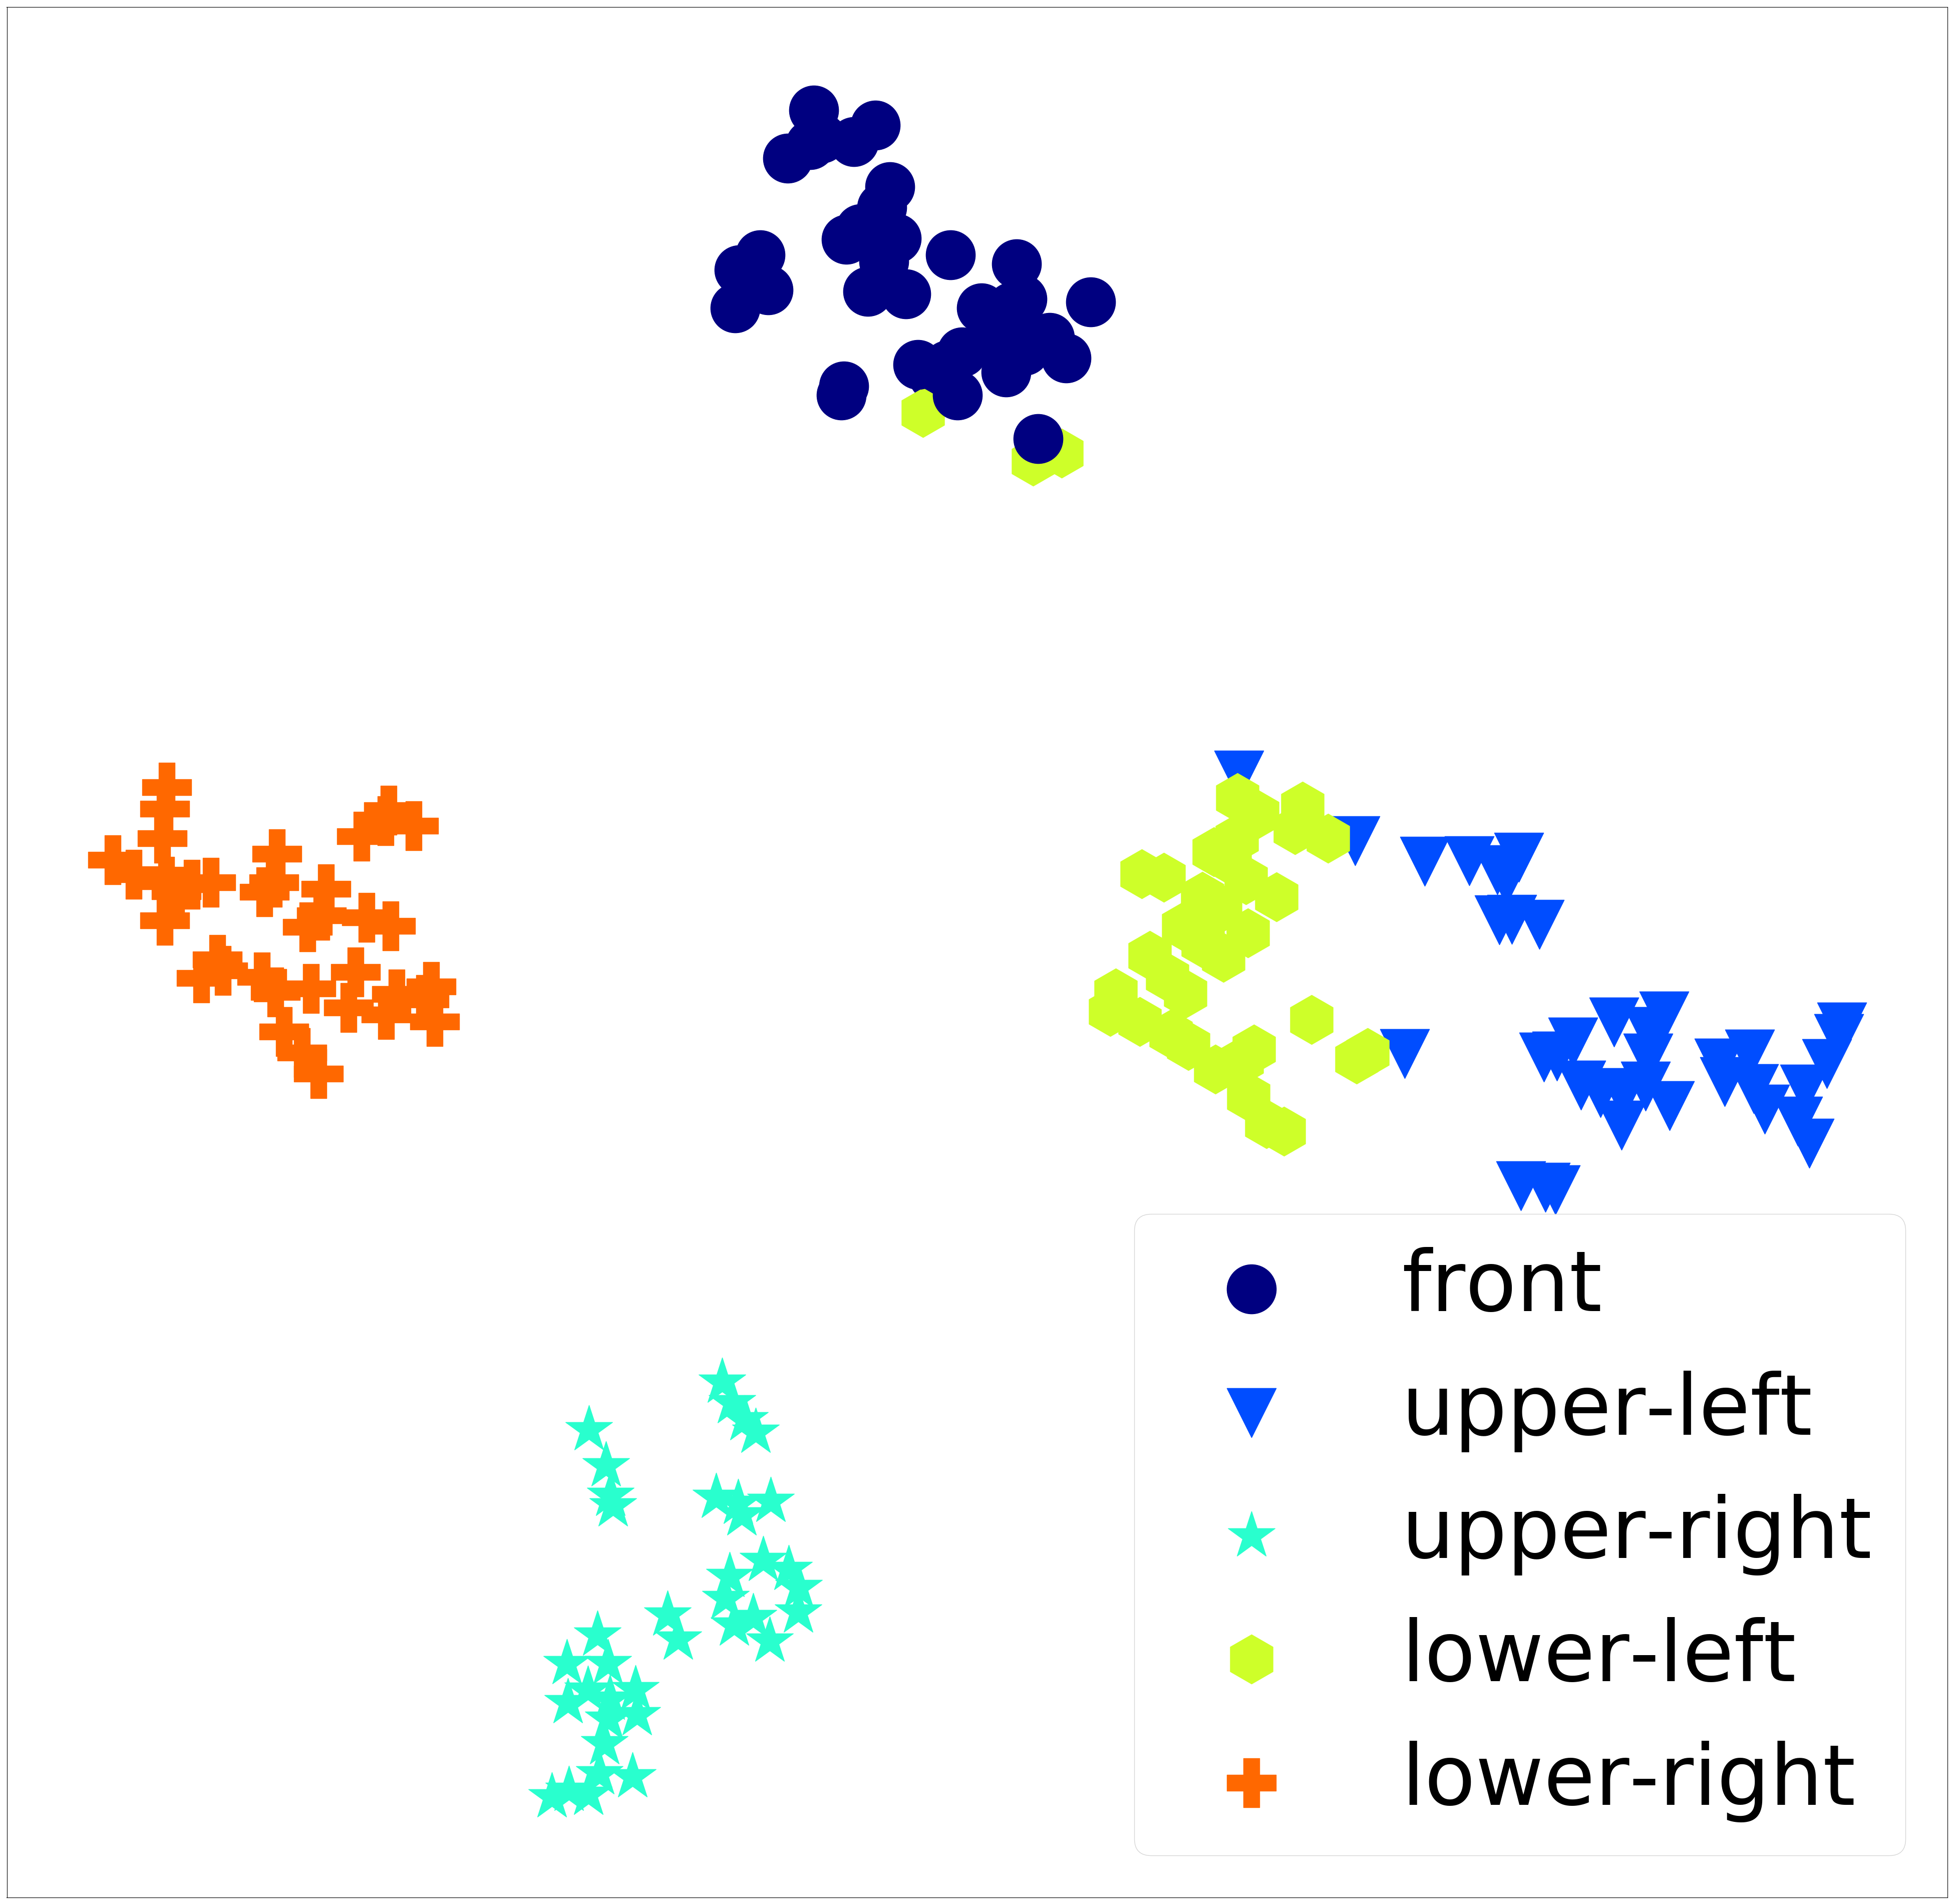
\includegraphics[width=\sfs\textwidth]{img/yaleb_raw_label.png}
\caption{}
\end{subfigure}
\begin{subfigure}{\fs\textwidth}
\centering
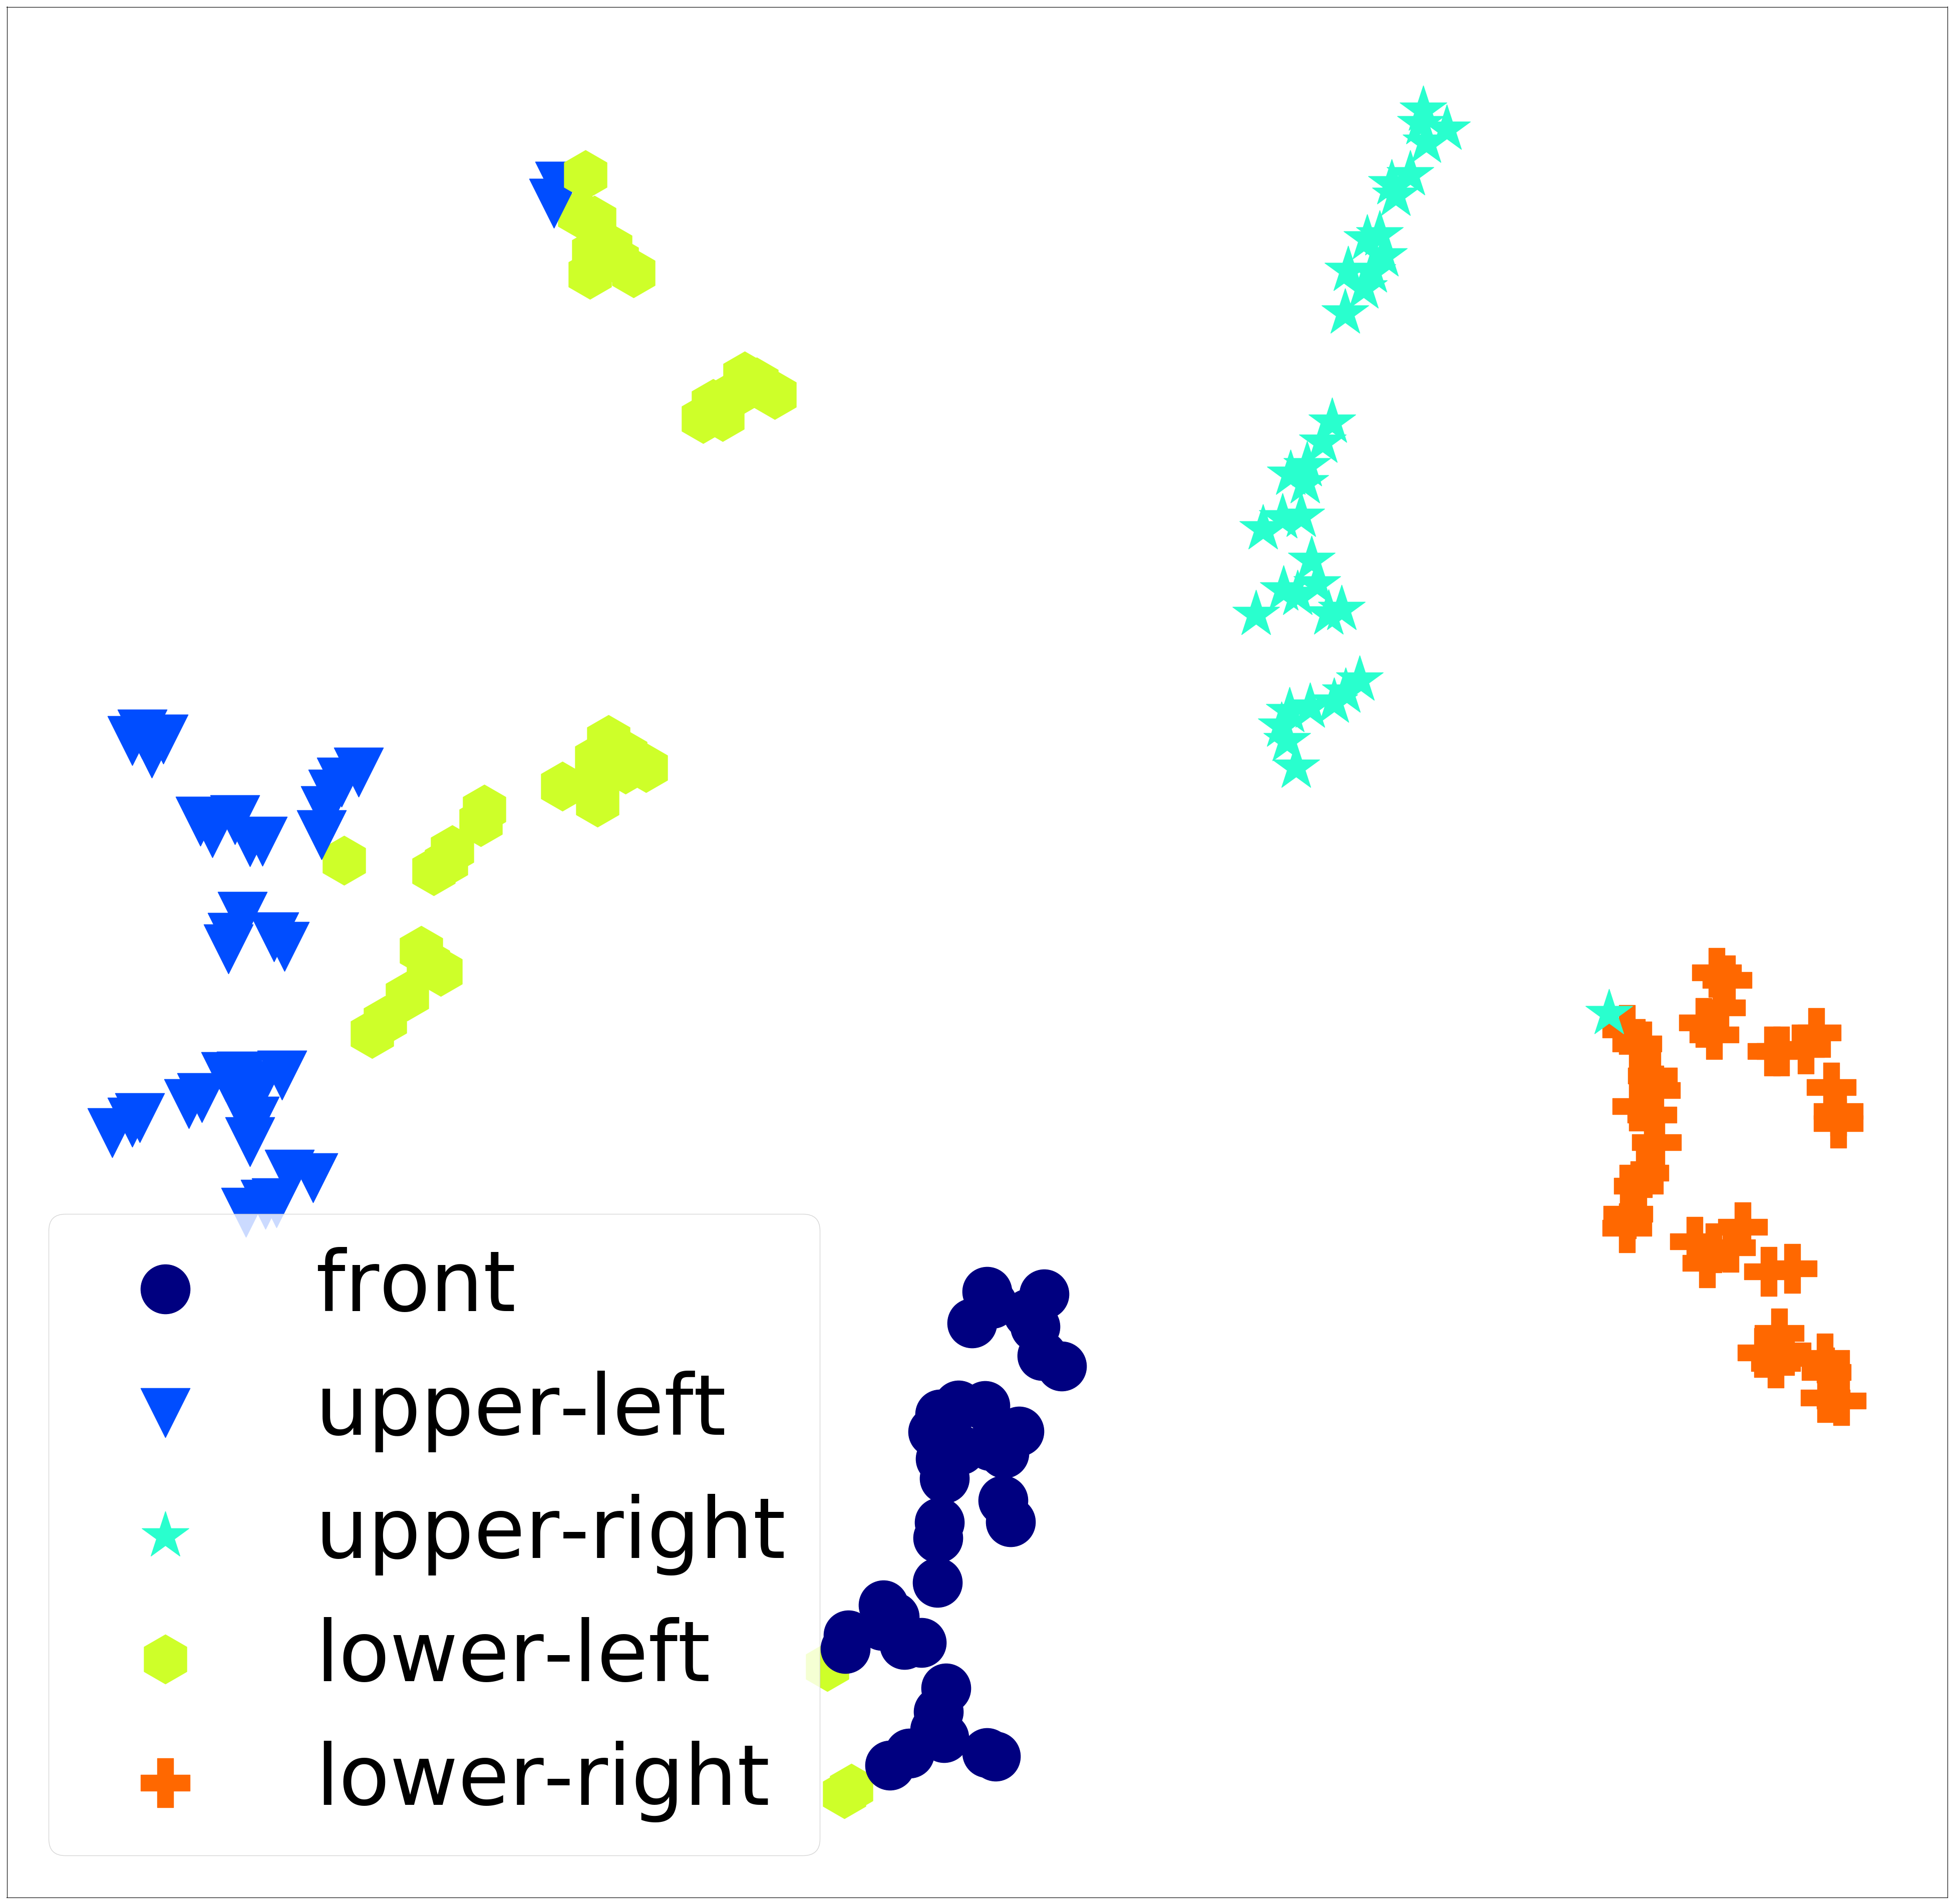
\includegraphics[width=\sfs\textwidth]{img/yaleb_e2_label.png}
\caption{}
\end{subfigure}
\begin{subfigure}{\fs\textwidth}
\centering
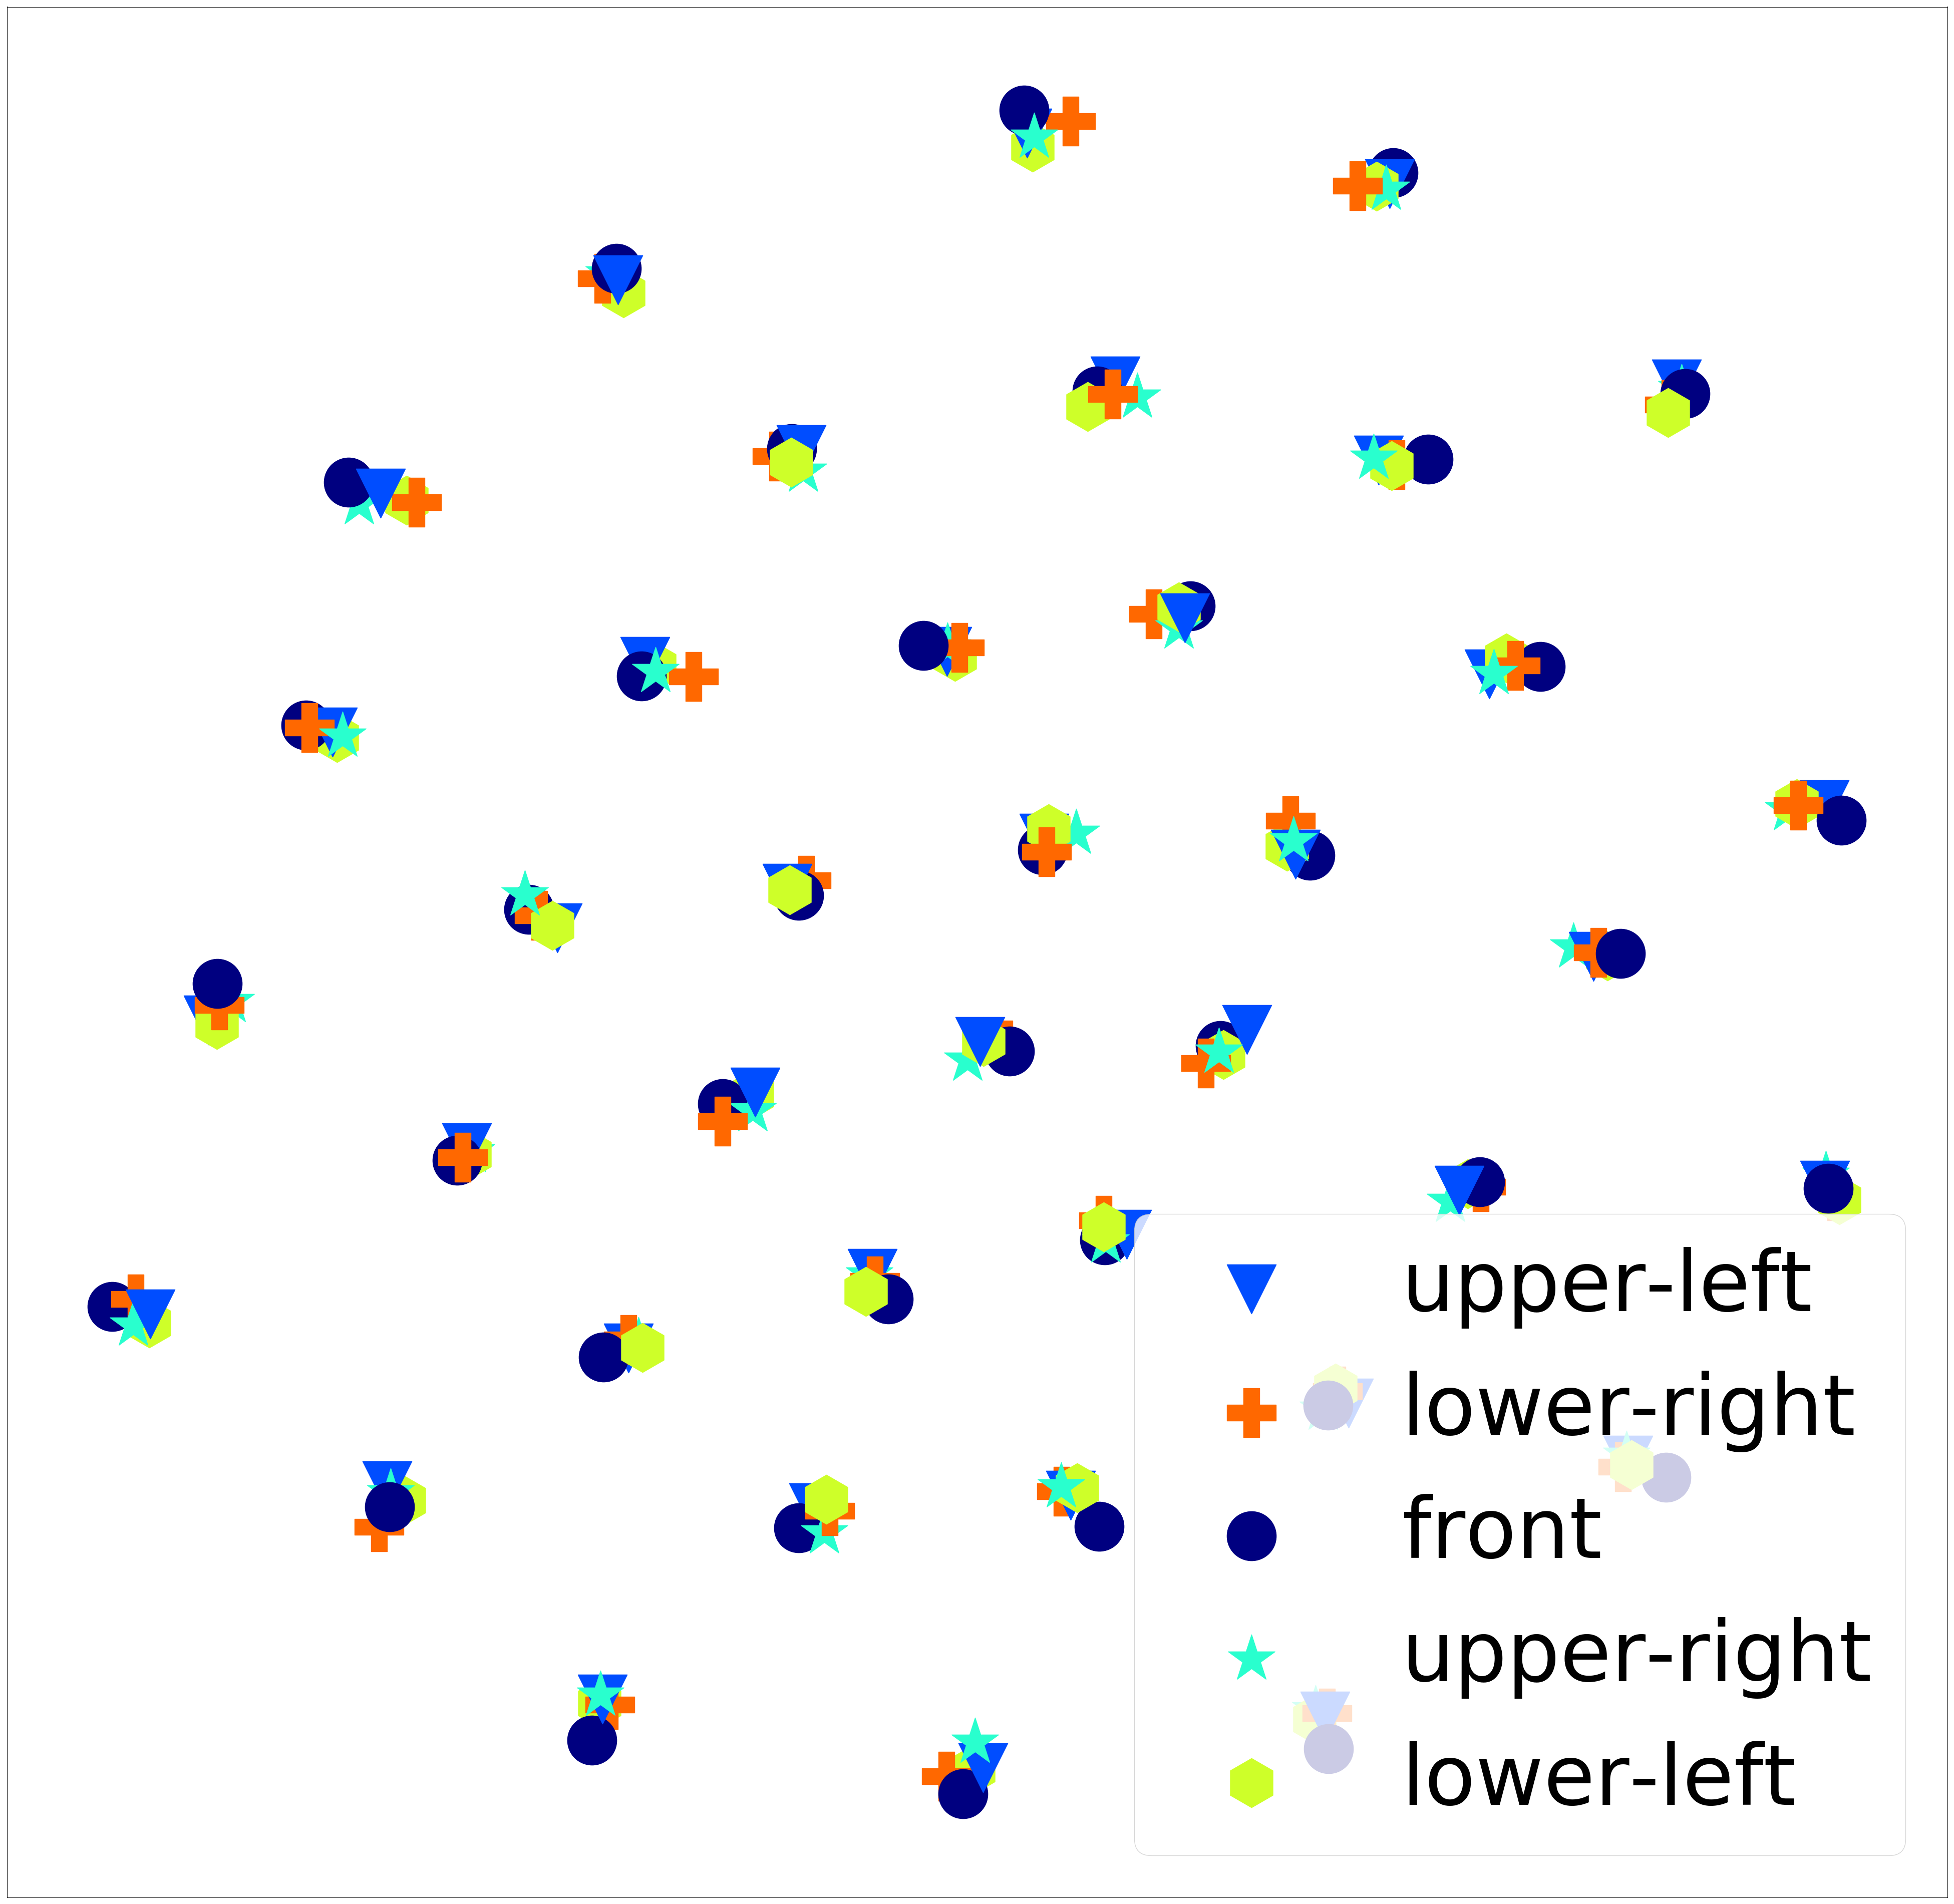
\includegraphics[width=\sfs\textwidth]{img/yaleb_e1_z.png}
\caption{}
\end{subfigure}
\begin{subfigure}{\fs\textwidth}
\centering
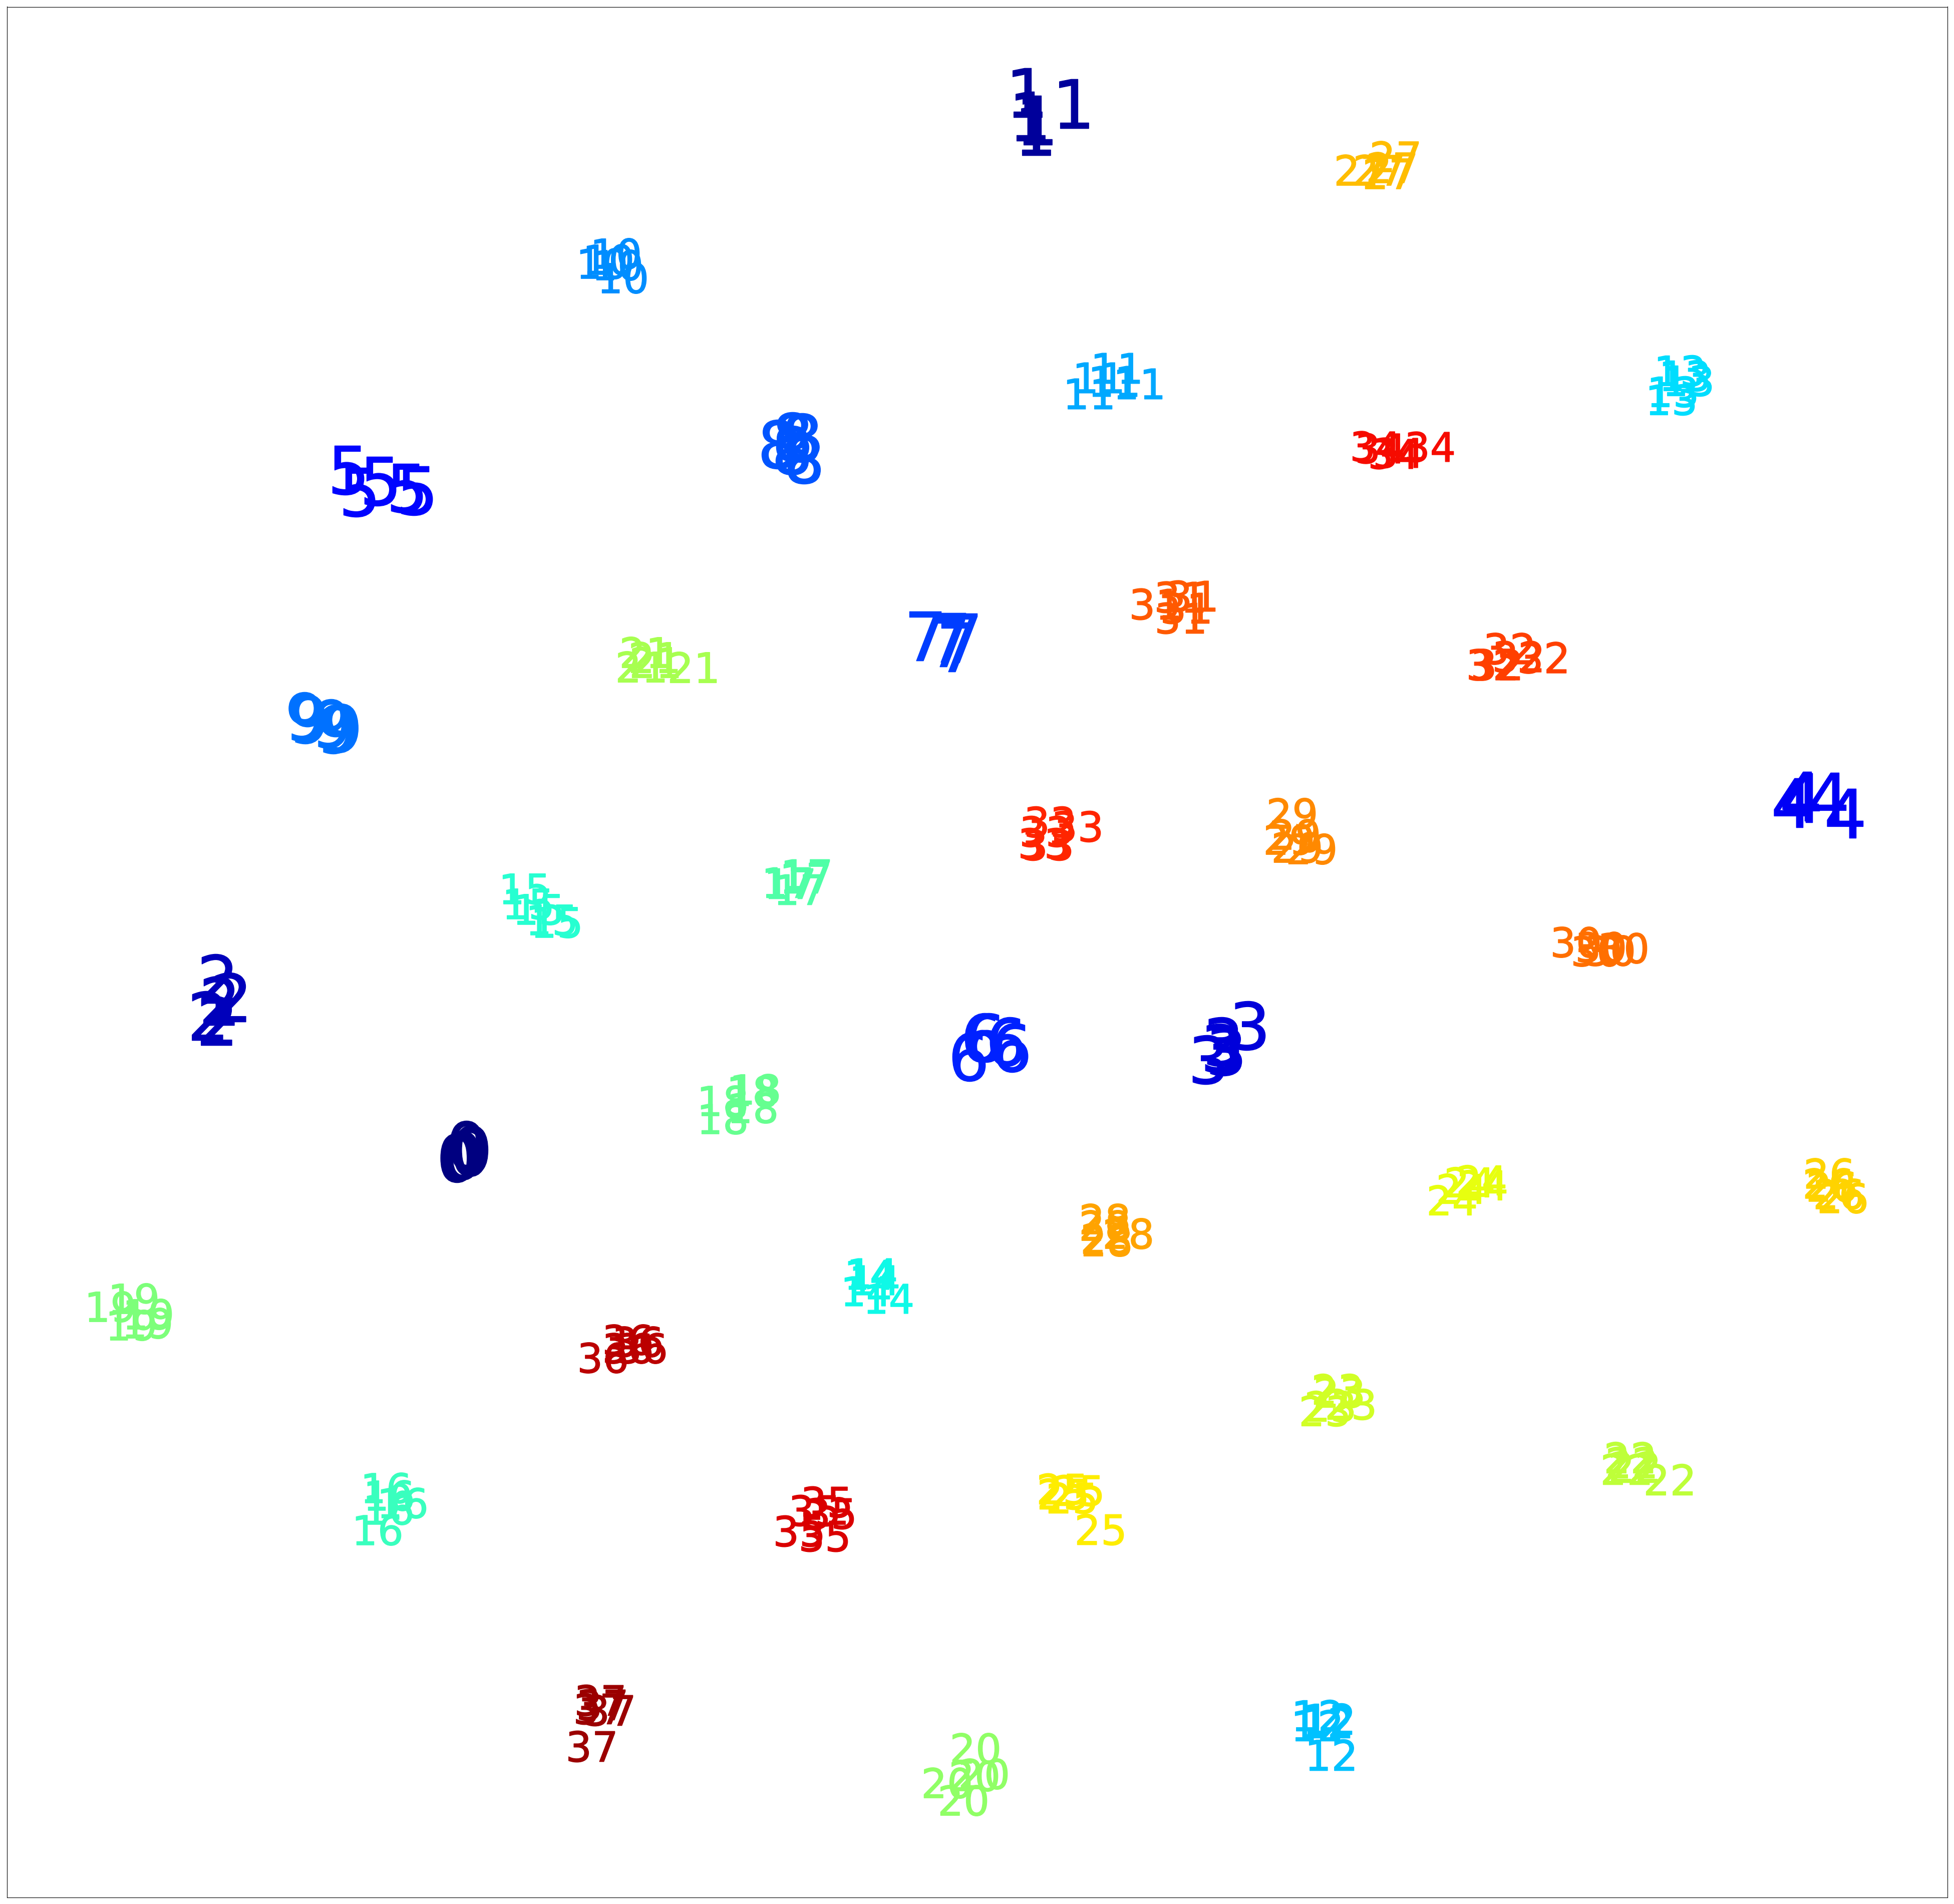
\includegraphics[width=\sfs\textwidth]{img/yaleb_e1_label.png}
\caption{}
\end{subfigure}
\caption{Extended Yale-B -- t-SNE visualization of (a) raw data, (b) $e_2$ labeled by lighting condition, (c) $e_1$ labeled by lighting condition, and (d) $e_1$ labeled by subject-ID (numerical markers, not colors).}
\label{fig:tsne_eyb}
\end{figure}
}

\section{Experimental Evaluation}
\label{sec:evaluation}

We provide experimental results on three tasks relevant to invariant feature learning for improved prediction of target variables: (1) invariance to inherent nuisance factors, (2) effective use of synthetic data augmentation for learning invariance, and (3) domain adaptation through learning invariance to ``domain'' information. We evaluate the performance of our model and prior works on two metrics -- accuracy of predicting $y$ from $e_1$ ($A_y$) and accuracy of predicting $z$ from $e_1$ ($A_z$). The goal of the model is to achieve high $A_y$ and $A_z$ close to random chance.

\begin{figure}
\captionsetup[subfigure]{aboveskip=1pt,belowskip=1pt}
\centering
\begin{subfigure}{0.85\textwidth}
\centering
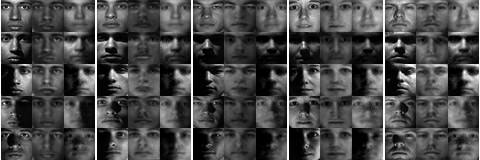
\includegraphics[width=\textwidth]{img/yaleb_recon.png}
\caption{\label{fig:recon_eyb}}
\end{subfigure}
\hfill
\begin{subfigure}{0.85\textwidth}
\centering
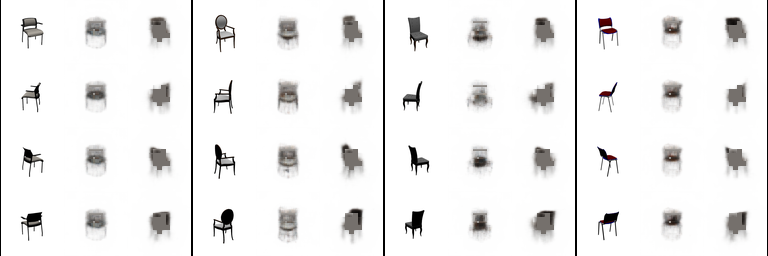
\includegraphics[width=\textwidth]{img/chairs_recon.png}
\caption{\label{fig:recon_chairs}}
\end{subfigure}

\caption{Reconstruction from $e_1$ and $e_2$ for (a) Extended Yale B and (b) Chairs. Columns in each block reflect (left to right): real, reconstruction from $e_1$ and that from $e_2$.}
\end{figure}

\subsection{Invariance to inherent nuisance factors}

We provide results of our framework at the task of learning invariance to inherent nuisance factors on two datasets -- Extended Yale-B~\cite{bib:eyb} and Chairs~\cite{bib:chairs}.

% \vspace{10pt}
% \begin{figure}
% \centering
% 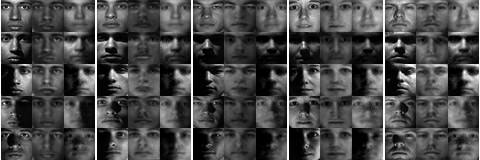
\includegraphics[width=0.7\textwidth]{img/yaleb_recon.png}
% \caption{\label{fig:recon_eyb}Extended Yale-B -- Reconstruction from $e_1$ and $e_2$. Columns in each block reflect (left to right): real, reconstruction from $e_1$ and that from $e_2$.}
% \end{figure}

% \begin{figure}
% \centering
% 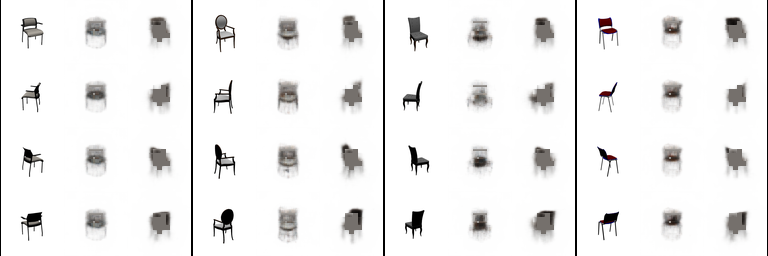
\includegraphics[width=0.7\textwidth]{img/chairs_recon.png}
% \caption{\label{fig:recon_chairs}Chairs -- Reconstruction from $e_1$ and $e_2$. Columns in each block reflect (left to right): real, reconstruction from $e_1$ and that from $e_2$.}
% \end{figure}

\textbf{Extended Yale-B.\quad} This dataset contains face-images of $38$ subjects under various lighting conditions. The target $y$ is the subject identity whereas the inherent nuisance factor $z$ is the lighting condition. We compare our framework to existing state-of-the-art supervised invariance induction methods, CAI~\cite{bib:sai}, VFAE~\cite{bib:vfae}, and NN+MMD~\cite{bib:nnmmd}. We use the prior works' version of the dataset, which has lighting conditions classified into five groups -- front, upper-left, upper-right, lower-left and lower-right, with the same split as $38 \times 5 = 190$ samples used for training and the rest used for testing~\cite{bib:nnmmd,bib:vfae,bib:sai}. We use the same architecture for the predictor and the encoder as CAI (as presented in~\cite{bib:sai}), i.e., single-layer neural networks, except that our encoder produces two encodings instead of one. We also model the decoder and the disentanglers as single-layer neural networks.

Table~\ref{tab:eyb} summarizes the results. The proposed unsupervised method outperforms existing state-of-the-art (supervised) invariance induction methods on both $A_y$ and $A_z$ metrics, providing a significant boost on $A_y$ and complete removal of lighting information from $e_1$ reflected by $A_z$. Furthermore, the accuracy of predicting $z$ from $e_2$ is $0.89$, which validates its automatic migration to $e_2$. Figure~\ref{fig:tsne_eyb} shows t-SNE~\cite{bib:tsne} visualization of raw data and embeddings $e_1$ and $e_2$ for our model. While raw data is clustered by lighting conditions $z$, $e_1$ exhibits clustering by $y$ with no grouping based on $z$, and $e_2$ exhibits near-perfect clustering by $z$. Figure~\ref{fig:recon_eyb} shows reconstructions from $e_1$ and $e_2$. Dedicated decoder networks were trained (with weights of $Enc$ frozen) to generate these visualizations. As evident, $e_1$ captures identity-related information but not lighting while $e_2$ captures the inverse.

% \begin{minipage}{\textwidth}
% \centering
% \begin{minipage}[c]{\textwidth}
% \centering
% % \captionsetup[subfigure]{font=scriptsize,labelfont=scriptsize,aboveskip=-1pt,belowskip=1pt}
% \begin{minipage}{0.6\textwidth}
% \centering
% 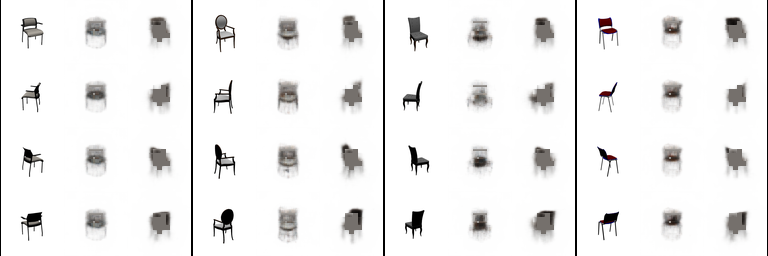
\includegraphics[width=\textwidth]{img/chairs_recon.png}
% \end{minipage}
% \captionsetup{aboveskip=5pt}
% \captionof{figure}{Chairs -- reconstruction from (a) $e_1$ and (b) $e_2$. Columns in each block reflect (left to right): real, reconstruction from $e_1$ and that from $e_2$.}
% \label{fig:recon_chairs}
% \end{minipage}
% % \hfill
% % \begin{minipage}[c]{0.27\textwidth}
% % \makegapedcells
% % \centering
% % \small
% % \begin{tabular}{ c ?{1.5pt} c ?{1.5pt} c }
% %   \hbline
% %   \textbf{Metric} & \textbf{CAI} & \textbf{Ours} \\
% %   \hbline
% %   $A_y$ & 0.68 & \textbf{0.74} \\
% %   $A_z$ & 0.66 & \textbf{0.0} \\
% %   \hbline
% % \end{tabular}
% % \captionof{table}{Results on Chairs}
% % \label{tab:chairs}
% % \end{minipage}
% \end{minipage}

\begin{minipage}{\textwidth}
\centering
\begin{minipage}[c]{0.72\textwidth}
\centering
% \captionsetup[subfigure]{font=scriptsize,labelfont=scriptsize,aboveskip=-1pt,belowskip=1pt}
\begin{minipage}{.47\textwidth}
\centering
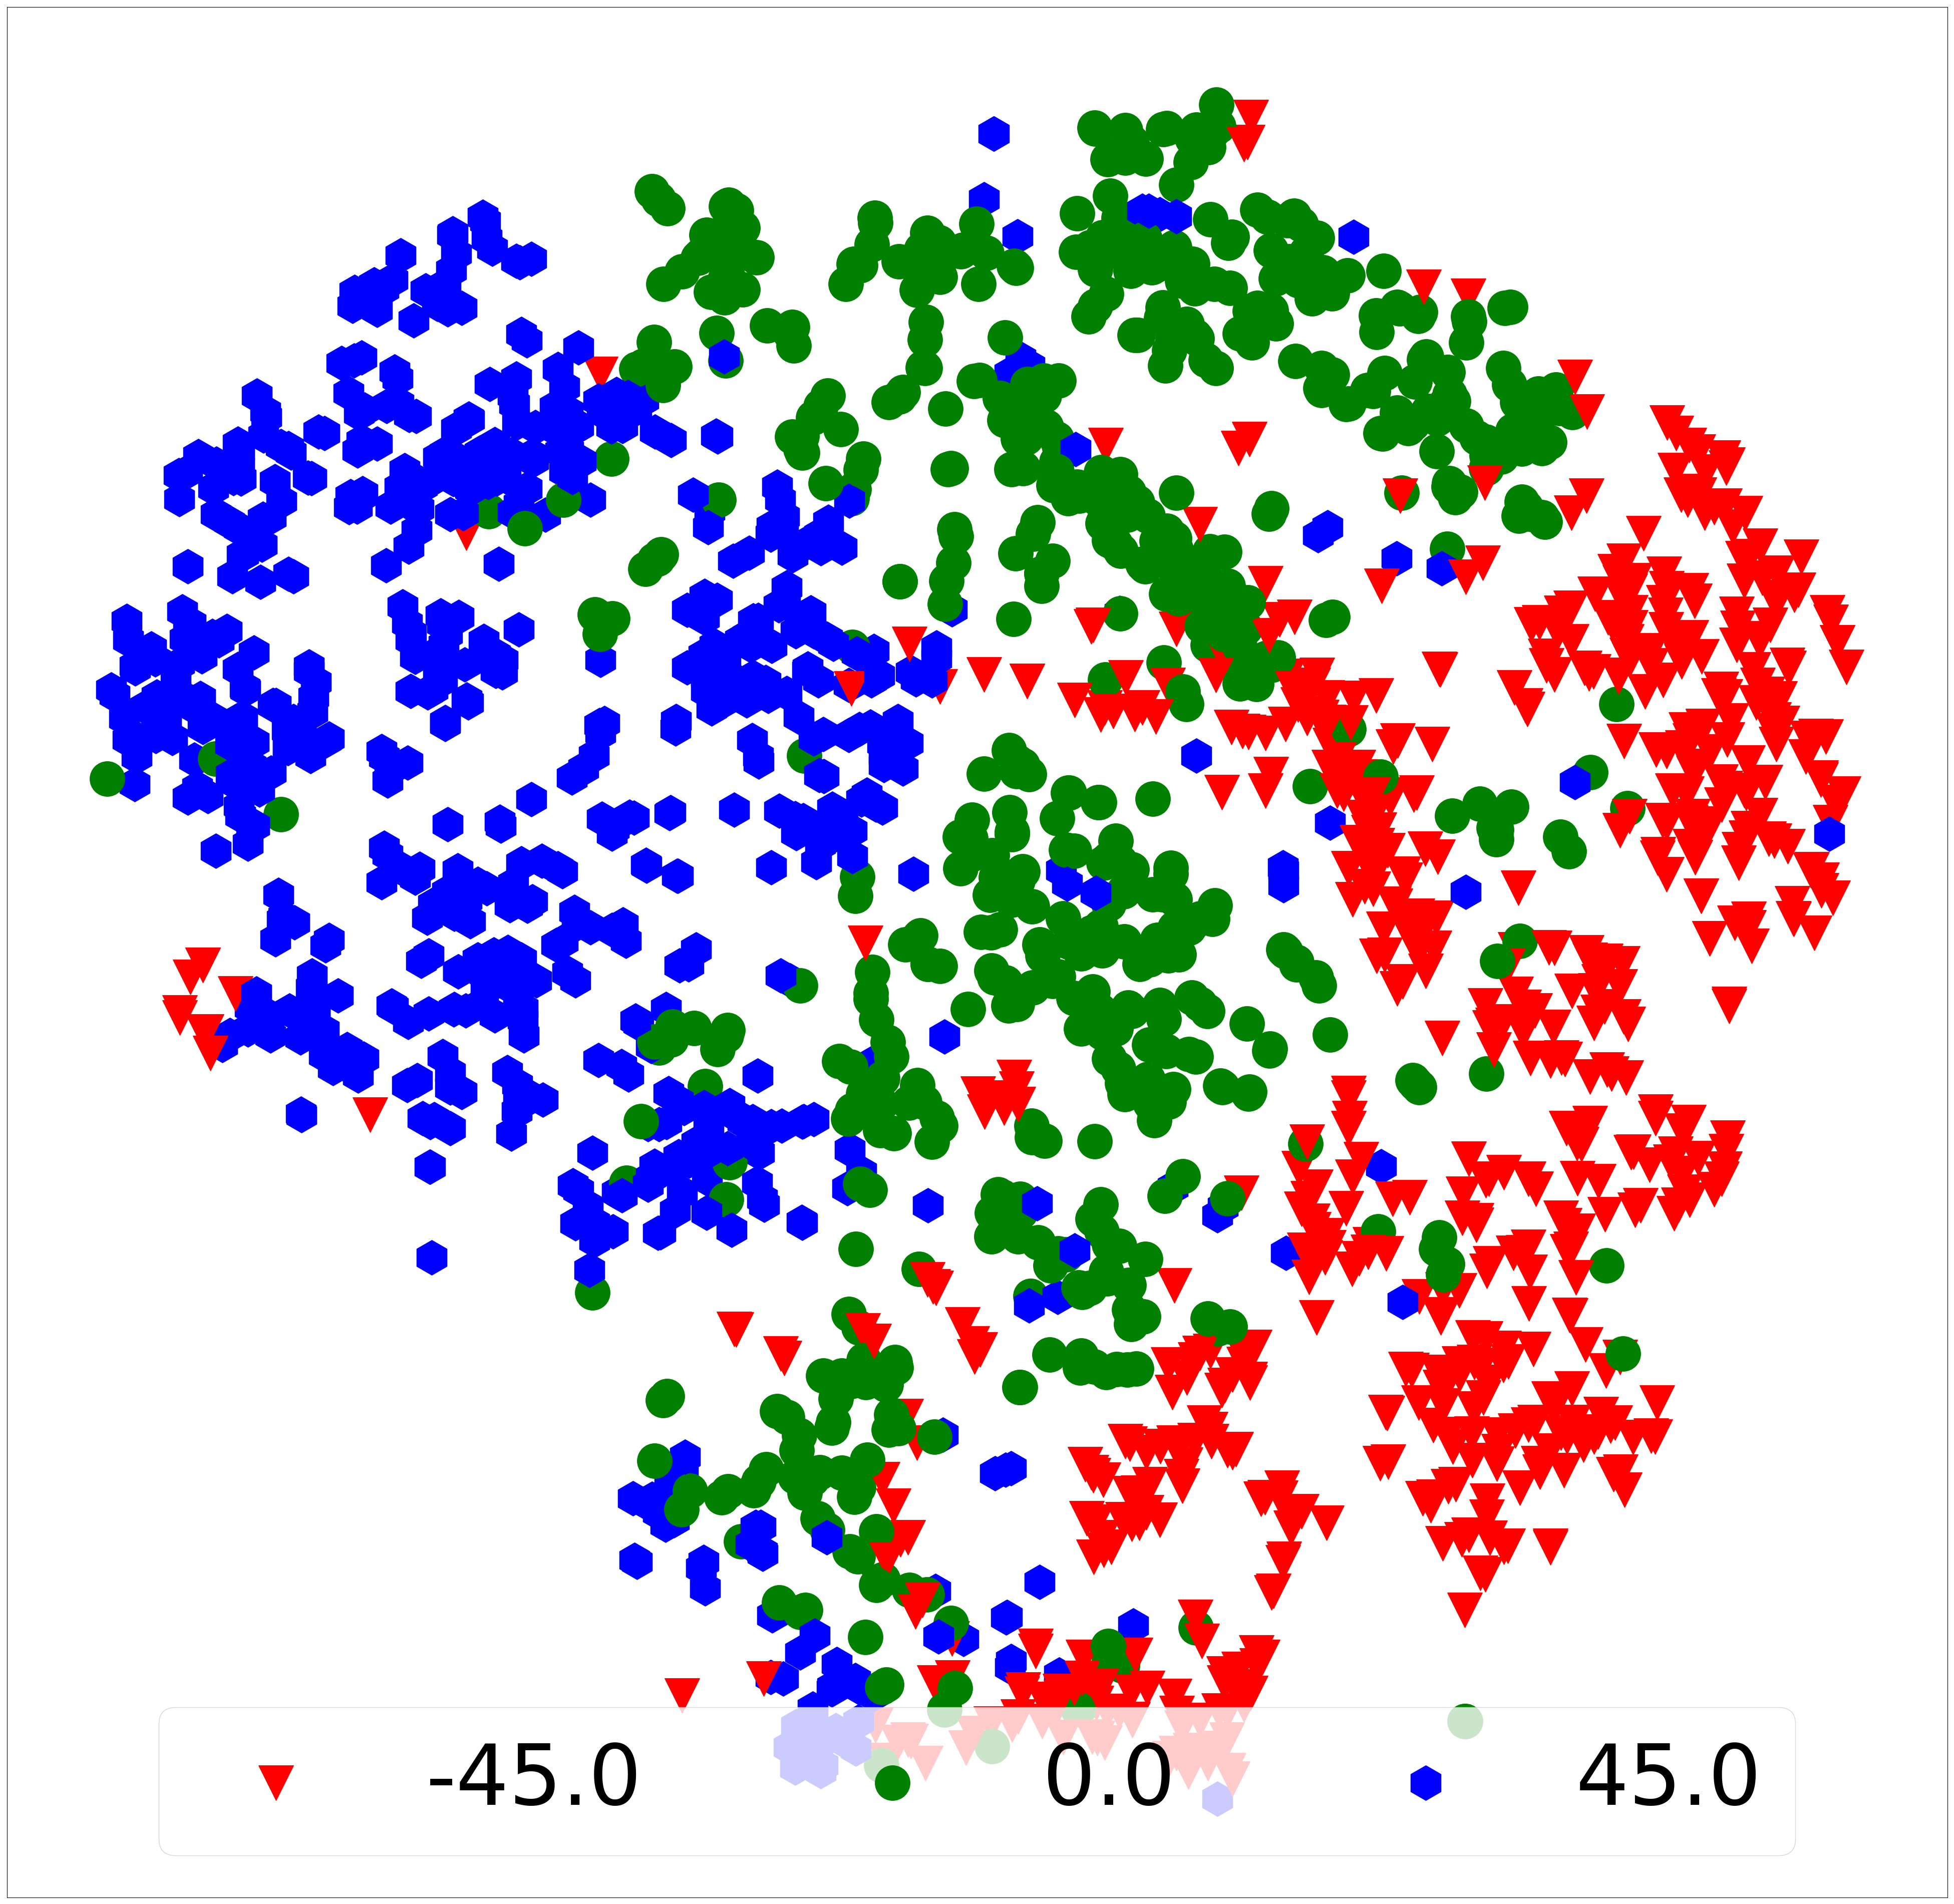
\includegraphics[width=0.75\textwidth]{img/mnist_rot_raw_label.png}
\captionsetup{aboveskip=1pt,belowskip=-5pt}
\captionof*{figure}{(a)}
\end{minipage}
\begin{minipage}{.47\textwidth}
\centering
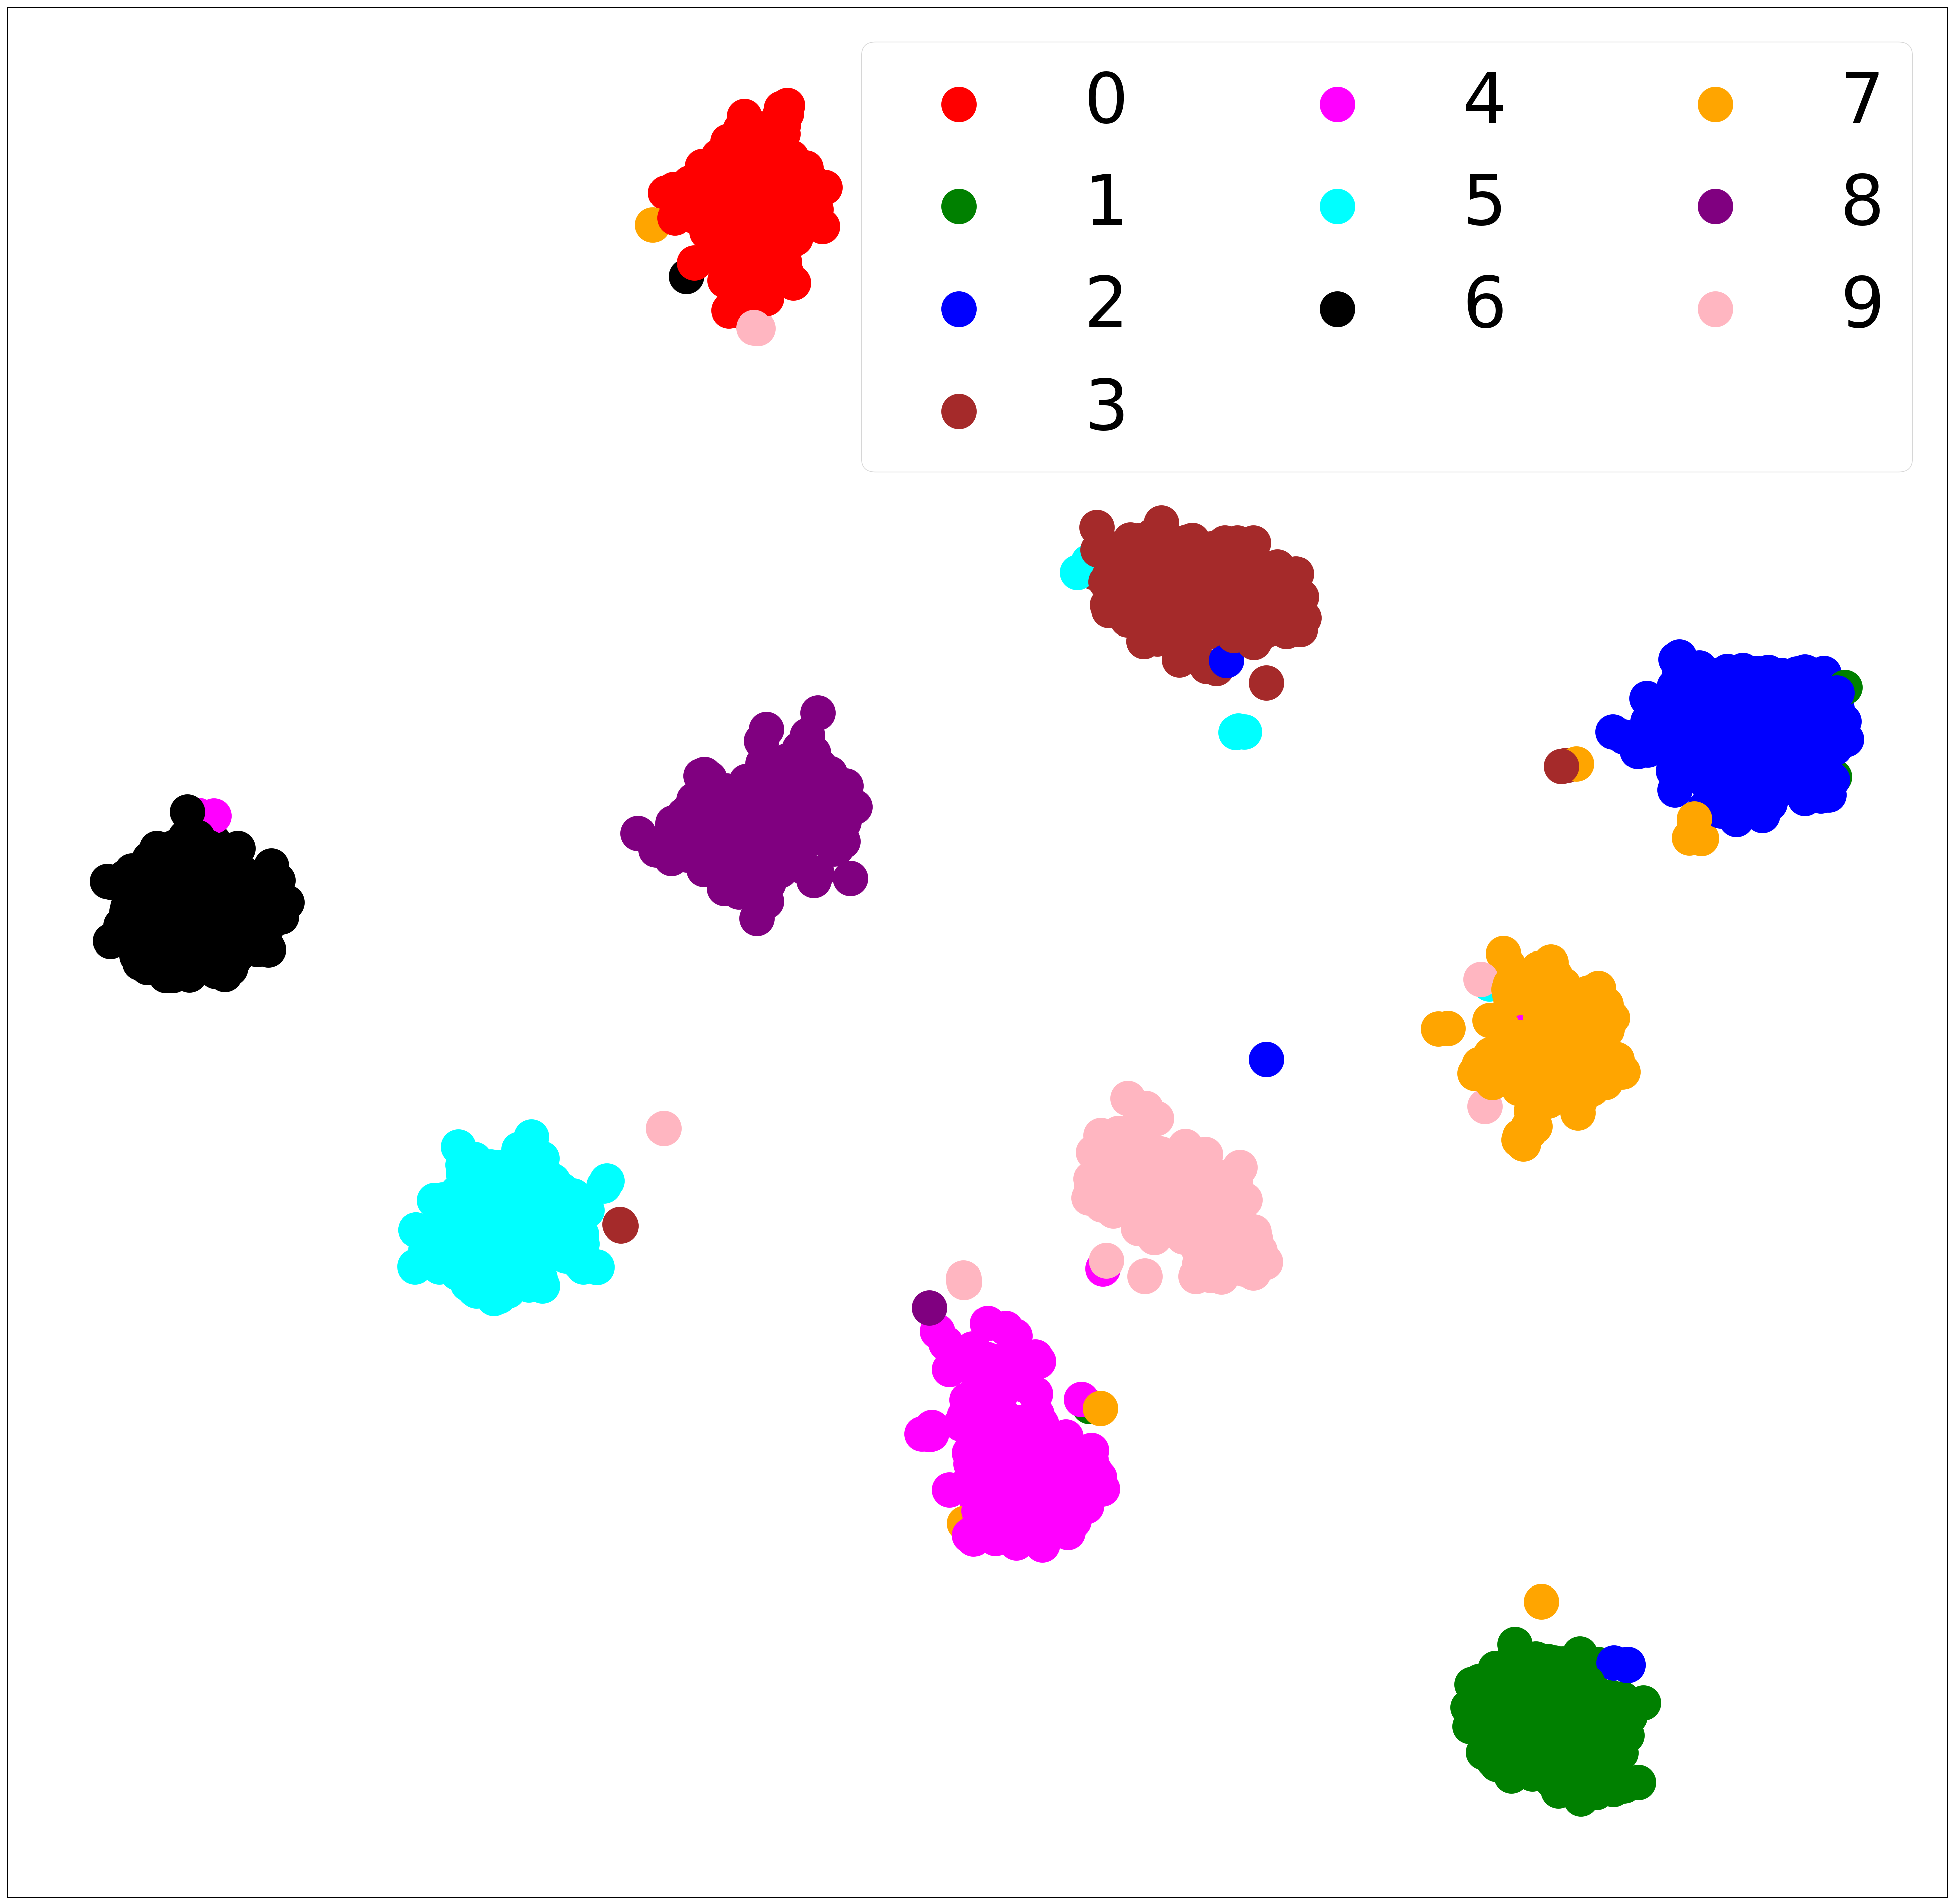
\includegraphics[width=0.75\textwidth]{img/mnist_rot_e1_label.png}
\captionsetup{aboveskip=1pt,belowskip=-5pt}
\captionof*{figure}{(b)}
\end{minipage}
\captionof{figure}{MNIST-ROT -- t-SNE visualization of (a) raw data and (b) $e_1$}
\label{fig:tsne_mnist_rot}
\end{minipage}
\hfill
\begin{minipage}[c]{0.27\textwidth}
\makegapedcells
\centering
\small
\begin{tabular}{ c ?{1.5pt} c ?{1.5pt} c }
  \hbline
  \textbf{Metric} & \textbf{CAI} & \textbf{Ours} \\
  \hbline
  $A_y$ & 0.68 & \textbf{0.74} \\
  $A_z$ & 0.69 & \textbf{0.34} \\
  \hbline
\end{tabular}
% \vspace{3pt}
\captionof{table}{\label{tab:chairs}Results on Chairs. High $A_y$ and low $A_z$ are desired.}
\end{minipage}
\end{minipage}

{
\def \fs {0.245}
\def \sfs {1}
\begin{figure*}[h]
\centering
\captionsetup[subfigure]{aboveskip=1pt,belowskip=1pt}
\begin{subfigure}{\fs\textwidth}
\centering
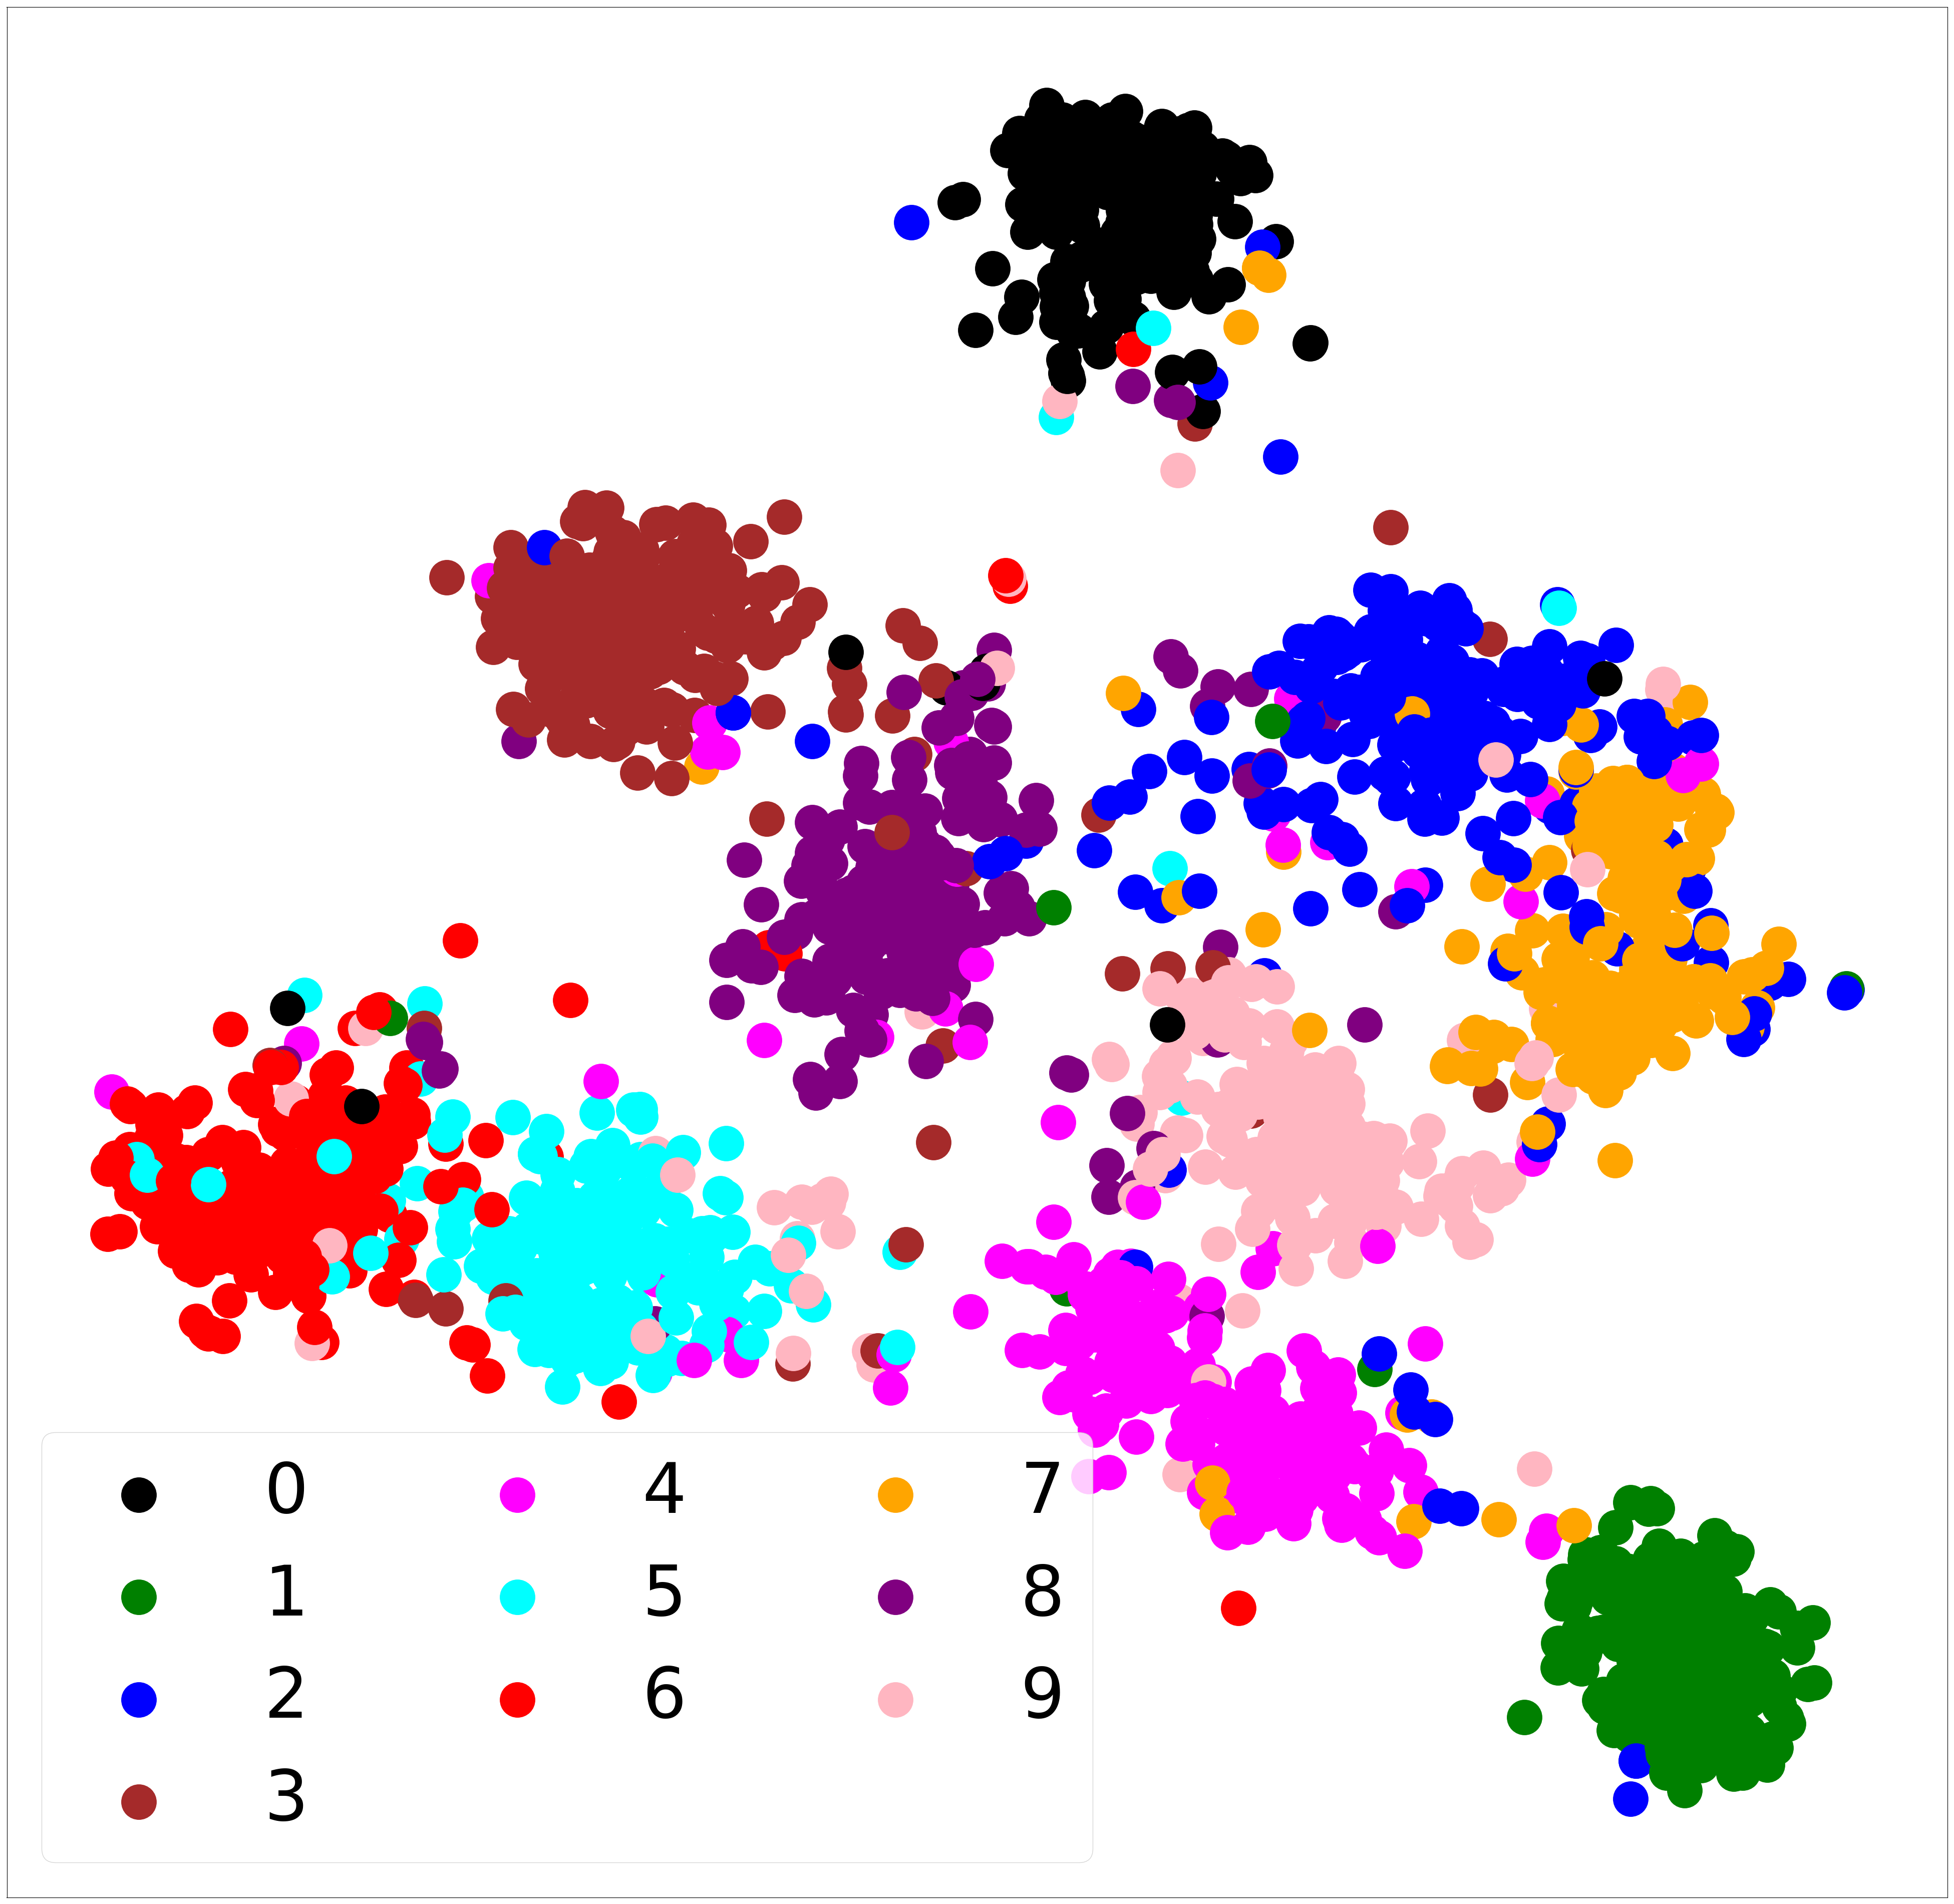
\includegraphics[width=\sfs\textwidth]{img/supp_mnist_rot_e1_label_55.png}
\caption{}
\end{subfigure}
\begin{subfigure}{\fs\textwidth}
\centering
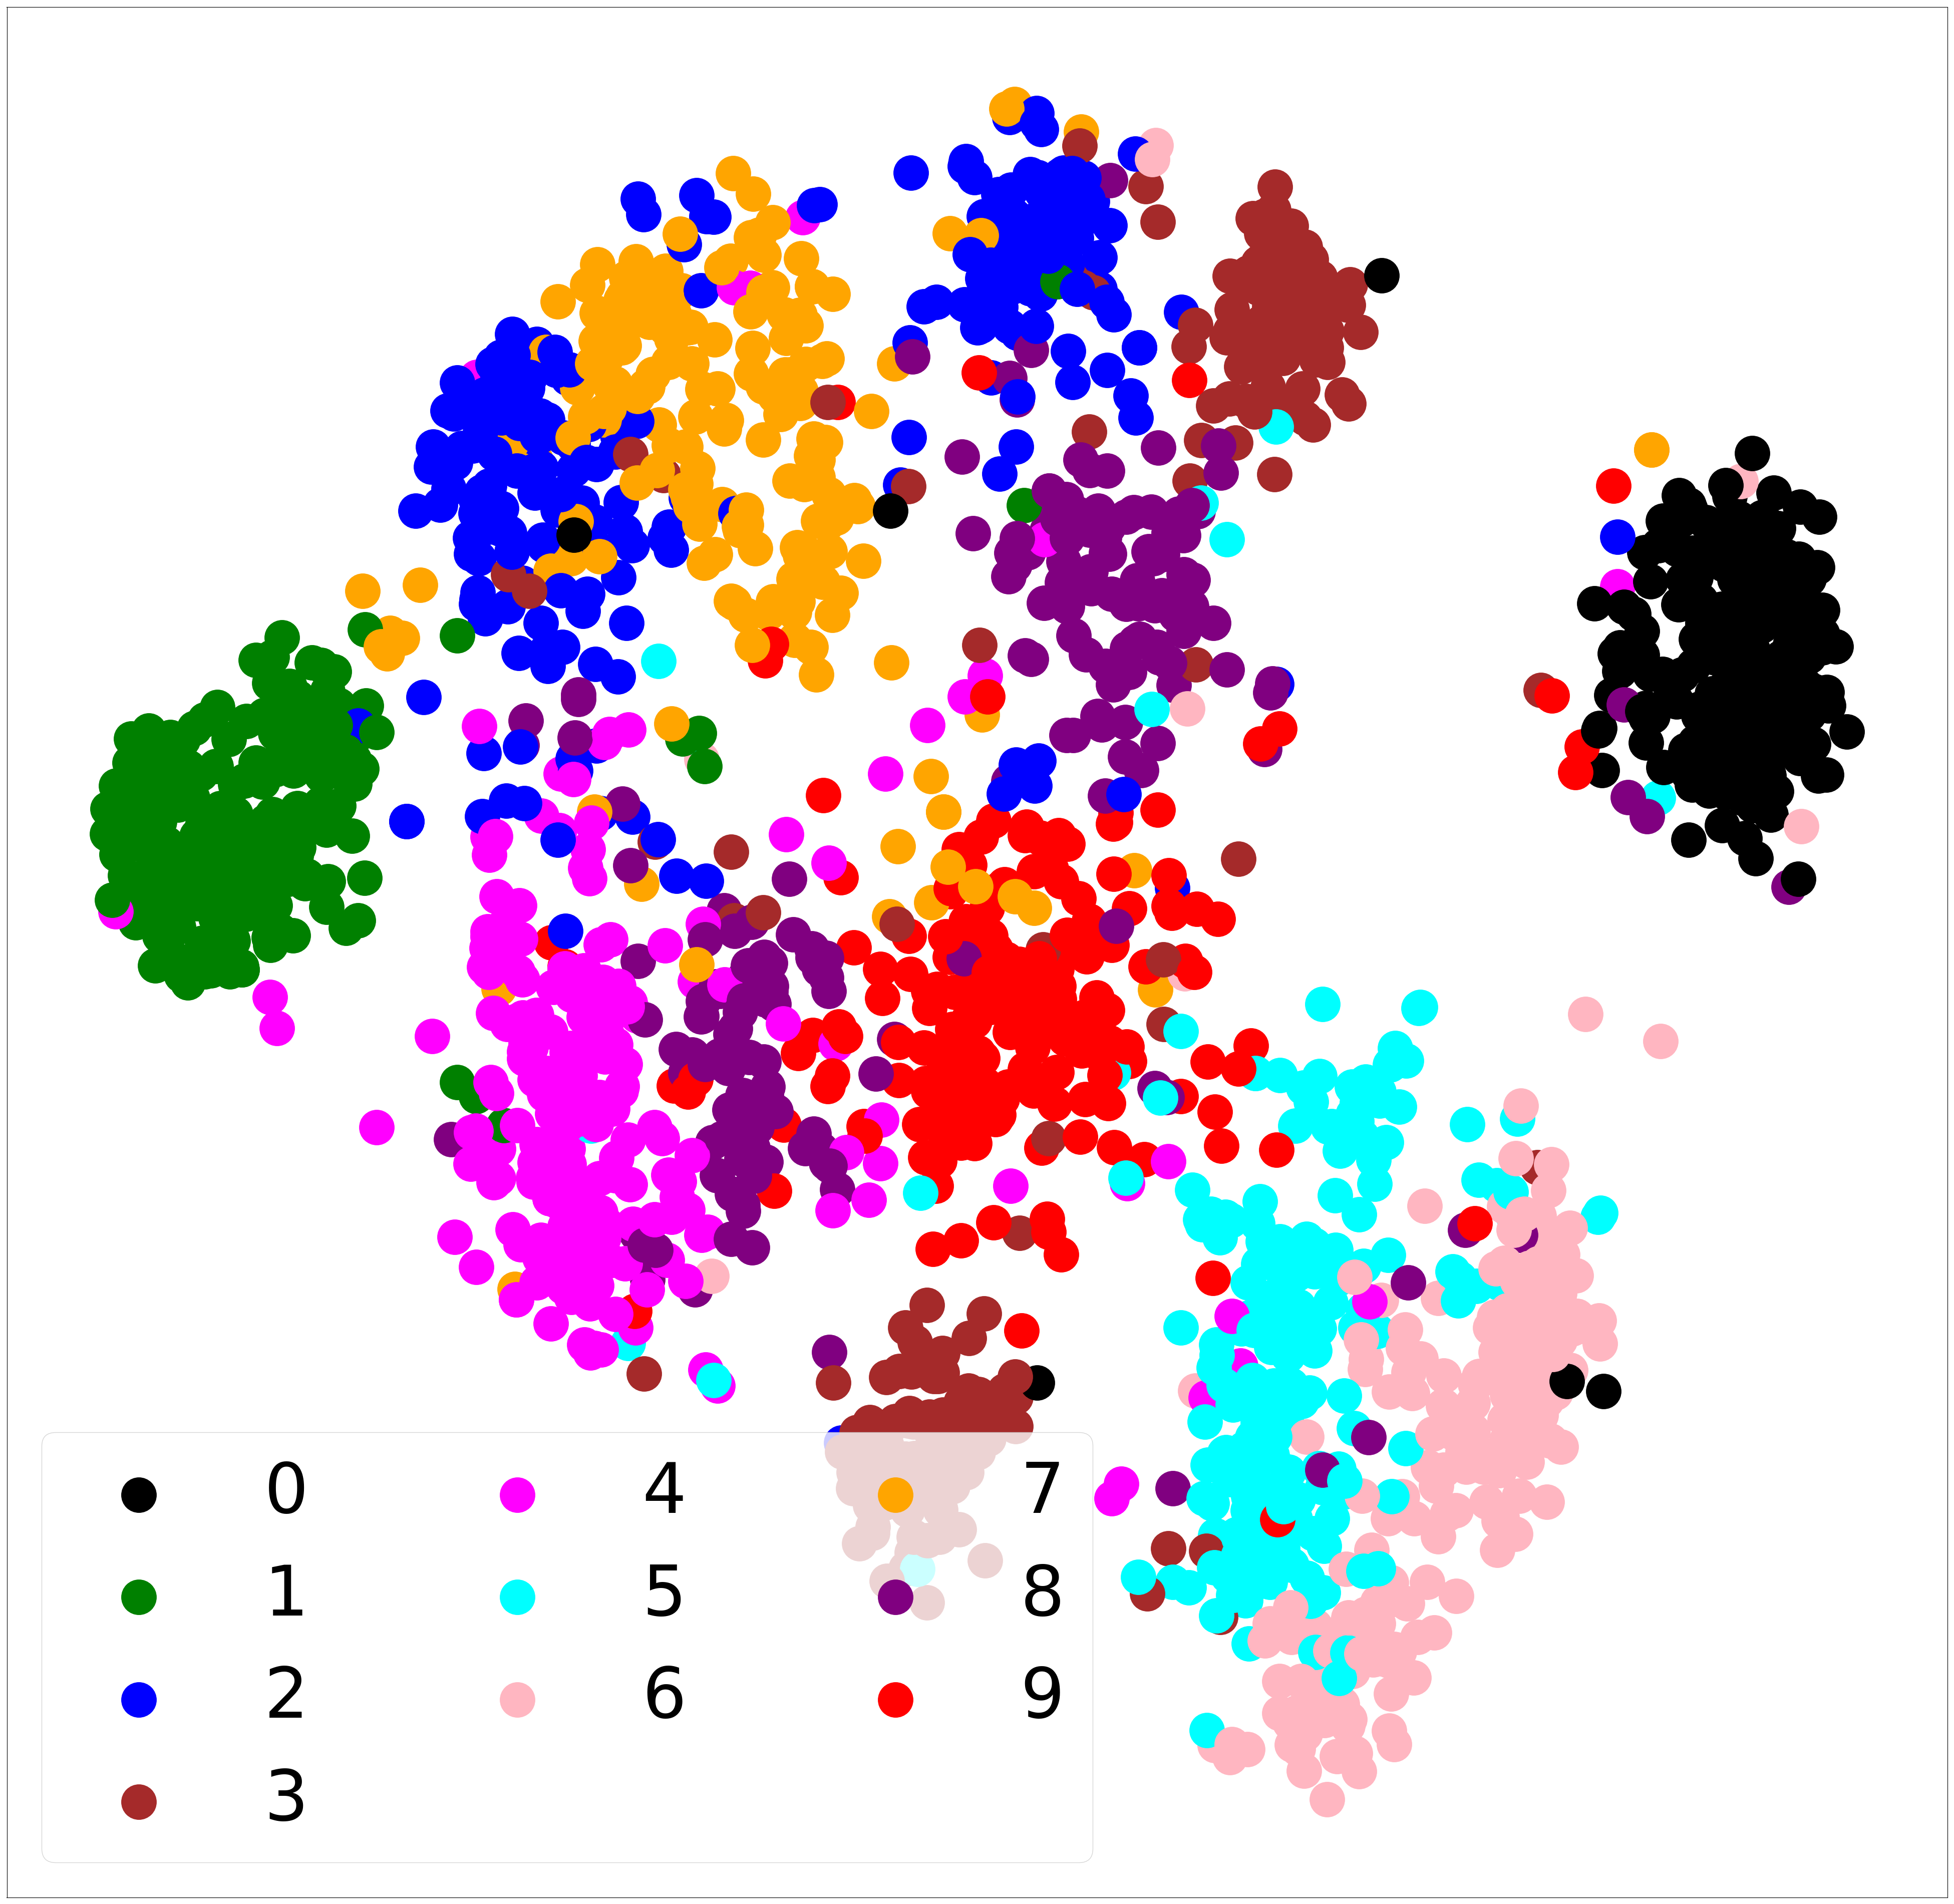
\includegraphics[width=\sfs\textwidth]{img/supp_mnist_rot_e1_label_55_b0.png}
\caption{}
\end{subfigure}
\begin{subfigure}{\fs\textwidth}
\centering
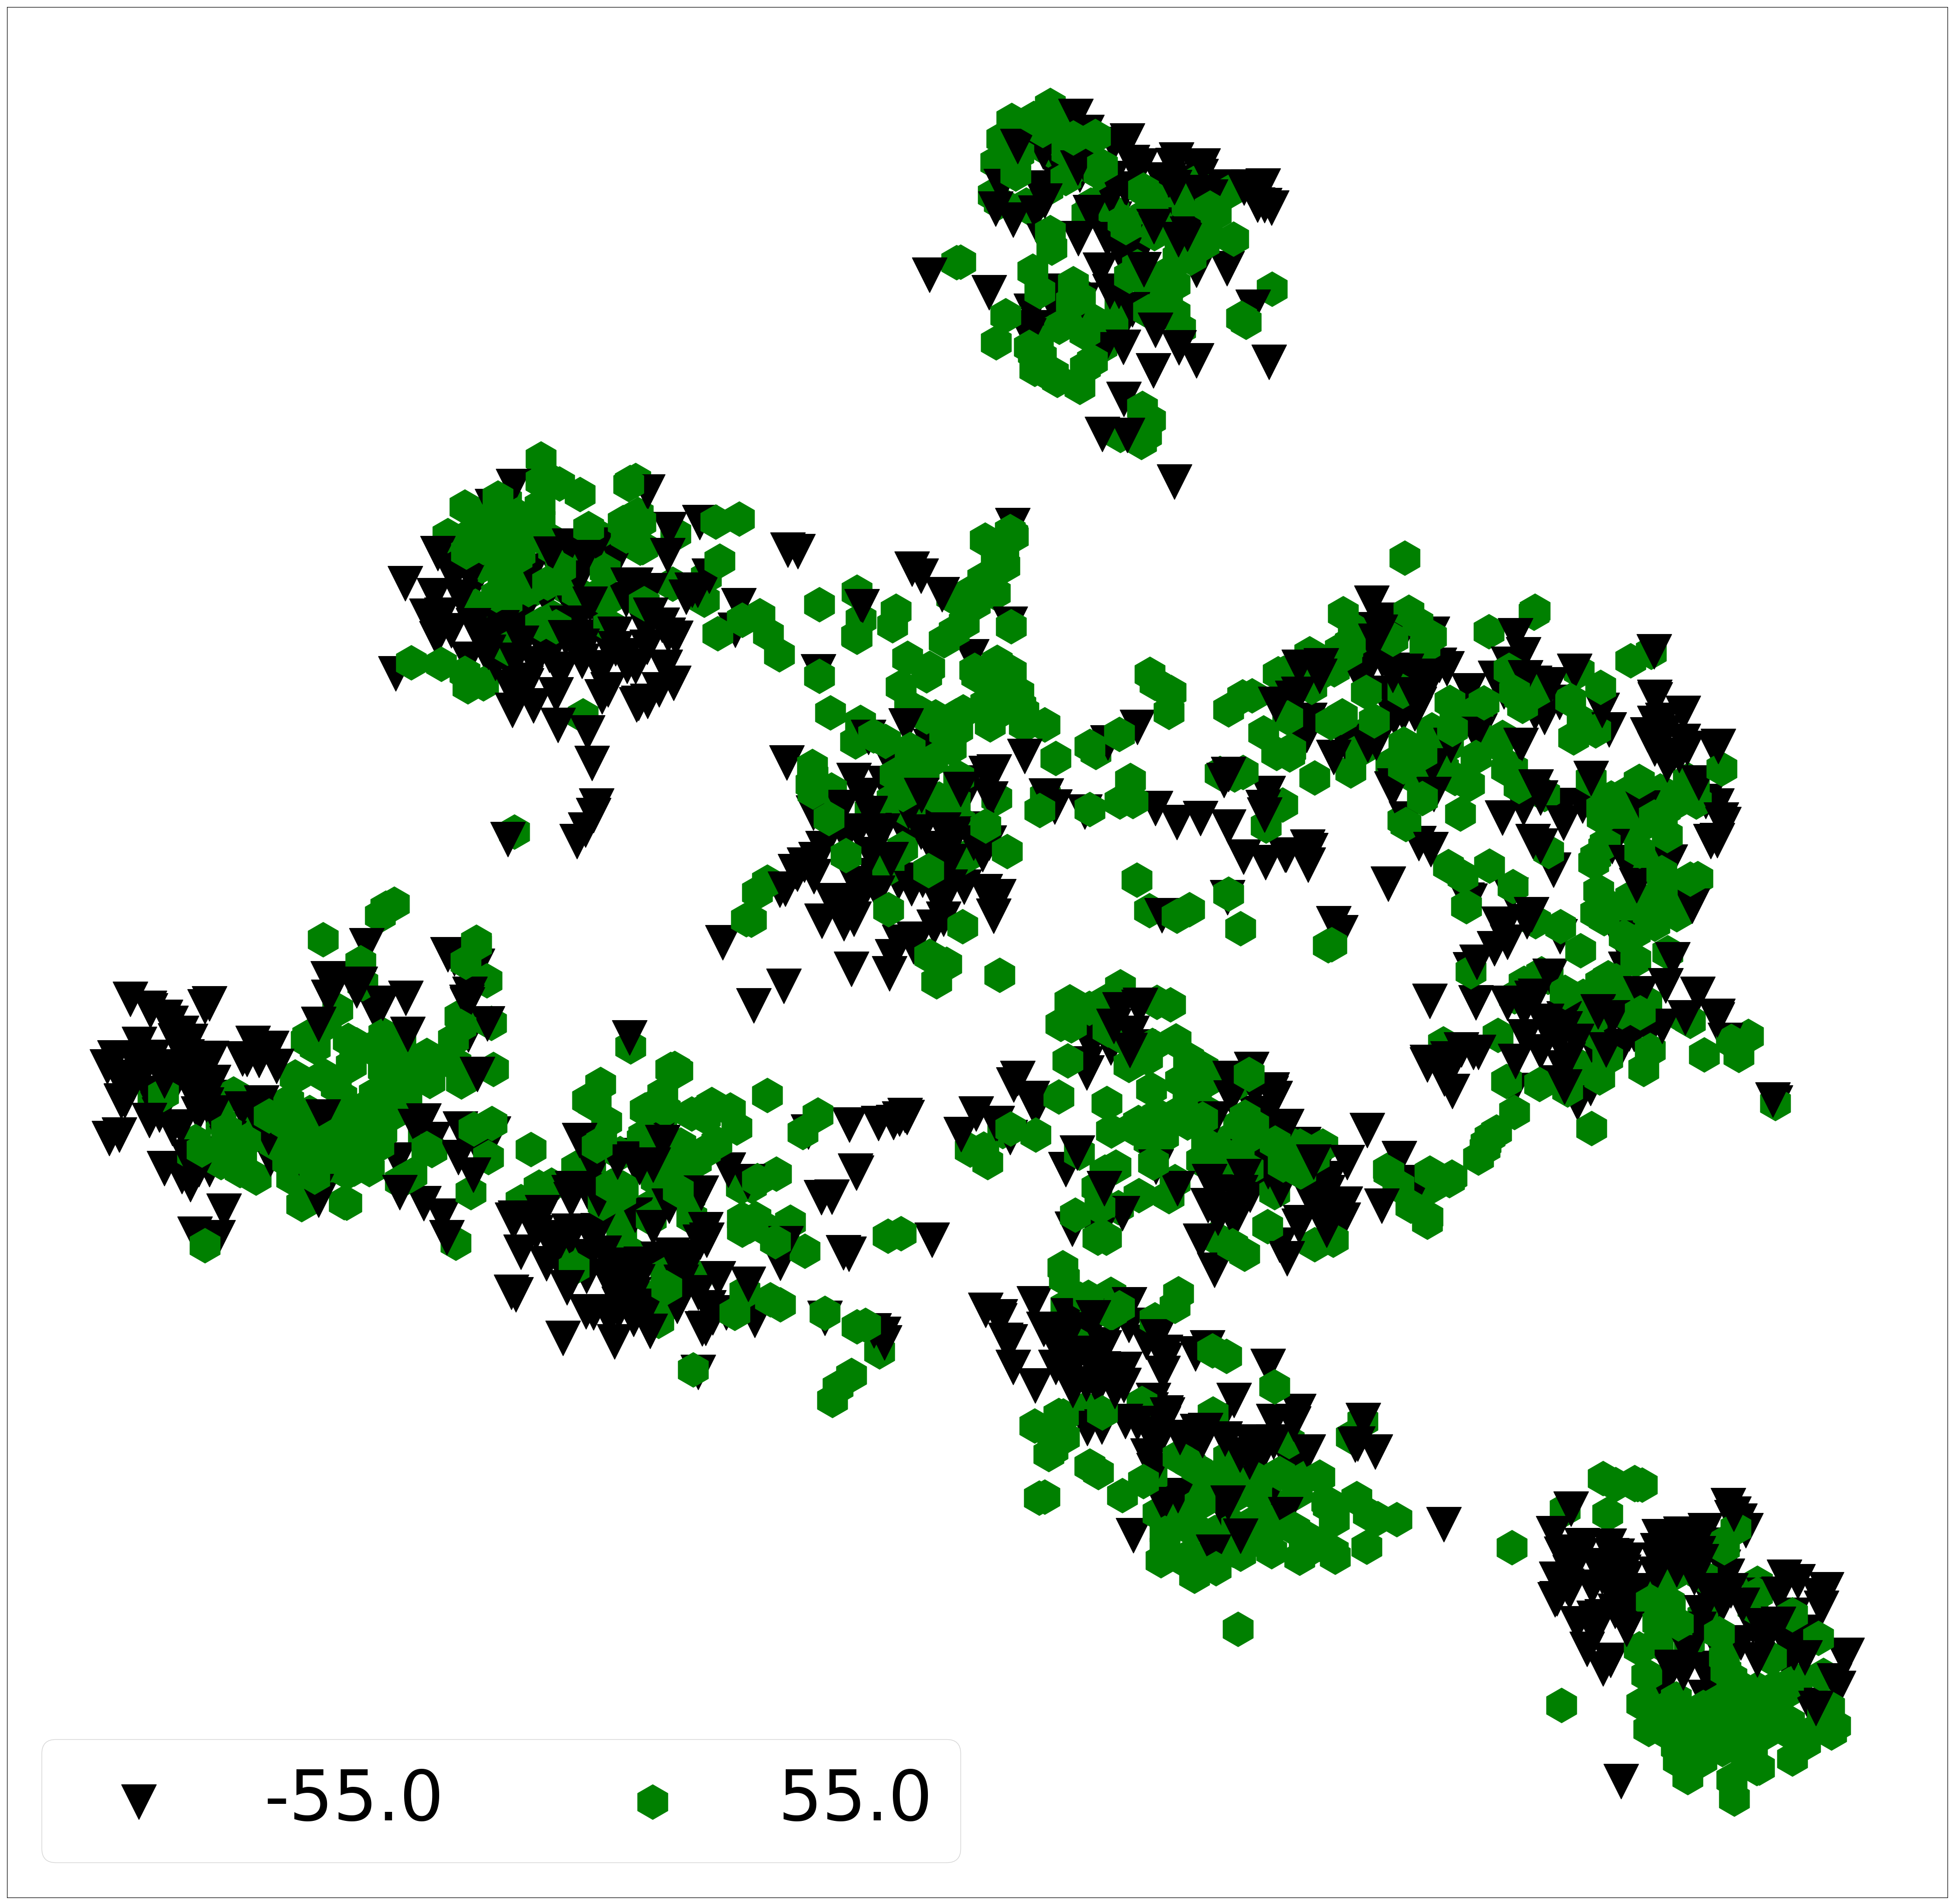
\includegraphics[width=\sfs\textwidth]{img/supp_mnist_rot_e1_label_55_z.png}
\caption{}
\end{subfigure}
\begin{subfigure}{\fs\textwidth}
\centering
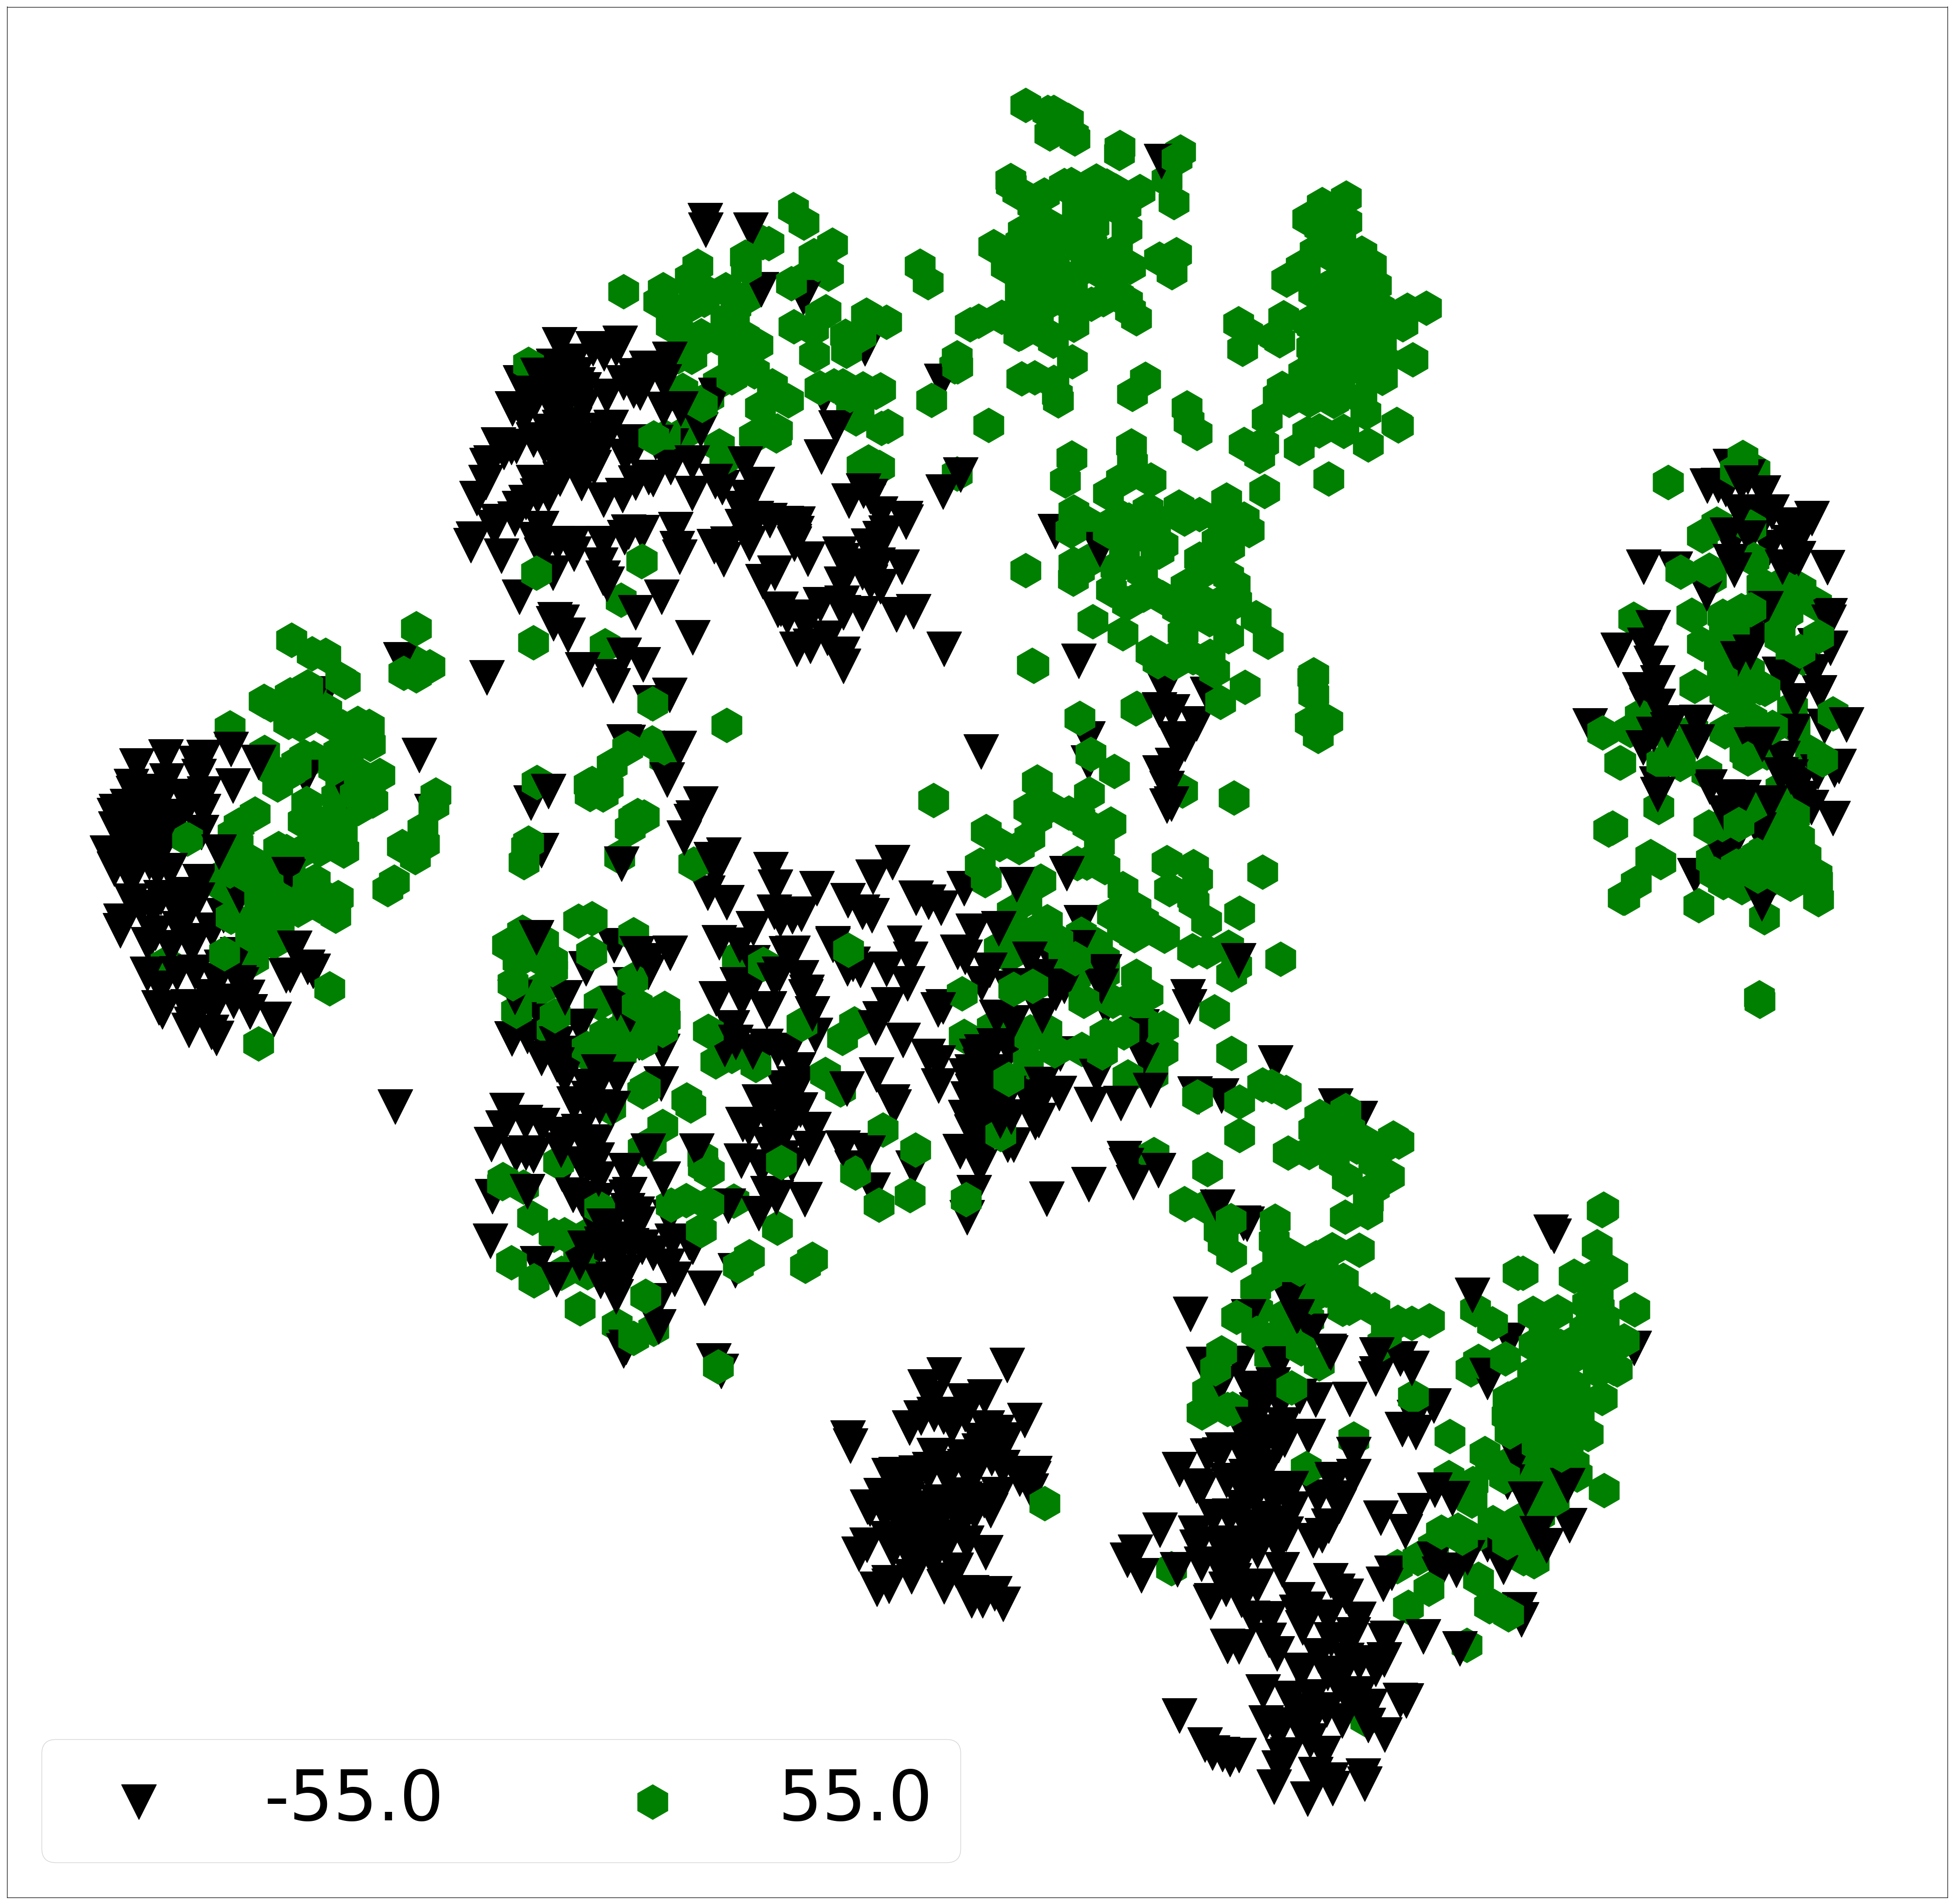
\includegraphics[width=\sfs\textwidth]{img/supp_mnist_rot_e1_label_55_z_b0.png}
\caption{}
\end{subfigure}
\caption{\label{fig:e1_55}t-SNE visualization of MNIST-ROT $e_1$ embedding for the proposed Unsupervised Adversarial Invariance model (a) \& (c), and baseline model $B_0$ (b) \& (d). Models trained on $\Theta = \{0, \pm22.5, \pm45\}$. Visualization generated for $\Theta = \{\pm55\}$.}
\end{figure*}
}

% \subsubsection{Chairs}

\vspace{10pt}
\textbf{Chairs.\quad} This dataset consists of $1393$ different chair types rendered at $31$ yaw angles and two pitch angles using a computer aided design model. We treat the chair identity as the target $y$ and the yaw angle $\theta$ as $z$. We split the data into training and testing sets by picking alternate yaw angles. Therefore, \emph{there is no overlap of $\theta$ between the two sets}. We compare the performance of our model to CAI. In order to train the CAI model, we group $\theta$ into four categories -- front, left, right and back, and provide it this information as a one-hot encoded vector. We model the encoder and the predictor as two-layer neural networks for both CAI and our model. We also model the decoder as a two-layer network and the disentanglers as single-layer networks. Table~\ref{tab:chairs} summarizes the results, showing that our model outperforms CAI on both $A_y$ and $A_z$. Moreover, the accuracy of predicting $\theta$ from $e_2$ is $0.73$, which shows that this information migrates to $e_2$. Figure~\ref{fig:recon_chairs} shows results of reconstructing $x$ from $e_1$ and $e_2$ generated in the same way as for Extended Yale-B above. The figure shows that $e_1$ contains identity information but nothing about $\theta$ while $e_2$ contains $\theta$ with limited identity information.

\subsection{Effective use of synthetic data augmentation for learning invariance}

Data is often not available for all possible variations of nuisance factors. A popular approach to learn models robust to such expected yet unobserved or infrequently seen (during training) variations is data augmentation through synthetic generation using methods ranging from simple operations~\cite{bib:data_aug_1} like rotation and translation to Generative Adversarial Networks~\cite{bib:gan_aug,bib:gan} for synthesis of more realistic variations. The prediction model is then trained on the expanded dataset. The resulting model, thus, becomes robust to specific forms of variations of certain nuisance factors that it has seen during training. Invariance induction, on the other hand, aims to completely prevent prediction models from using information about nuisance factors. Data augmentation methods can be more effectively used for improving the prediction of $y$ by using the expanded dataset for inducing invariance by \emph{exclusion} rather than \emph{inclusion}. We use two variants of the MNIST~\cite{bib:mnist} dataset of handwritten digits to (1) show the advantage of unsupervised invariance induction at this task over its supervised variant through comparison with CAI, and (2) perform ablation experiments for our model to justify our framework design. We use the same two-layer architectures for the encoder and the predictor in both our model and CAI, except that our encoder generates two encodings instead of one. We model the decoder as a three-layer neural network and the disentanglers as single-layer neural networks. We train two baseline versions of our model for our ablation experiments -- $B_0$ composed of $Enc$ and $Pred$, i.e., a single feed-forward network $x \dashedrightarrow h \dashedrightarrow y$ and $B_1$, which is the same as the composite model $M_1$, i.e., the proposed model trained non-adversarially without the disentanglers. $B_0$ is used to validate the phenomenon that invariance by exclusion is a better approach than robustness through inclusion whereas $B_1$ helps evaluate the importance of disentanglement in our framework.

% \begin{figure}
% \captionsetup[subfigure]{font=scriptsize,labelfont=scriptsize,aboveskip=1pt,belowskip=1pt}
% \centering
% \begin{subfigure}{.275\textwidth}
% \centering
% 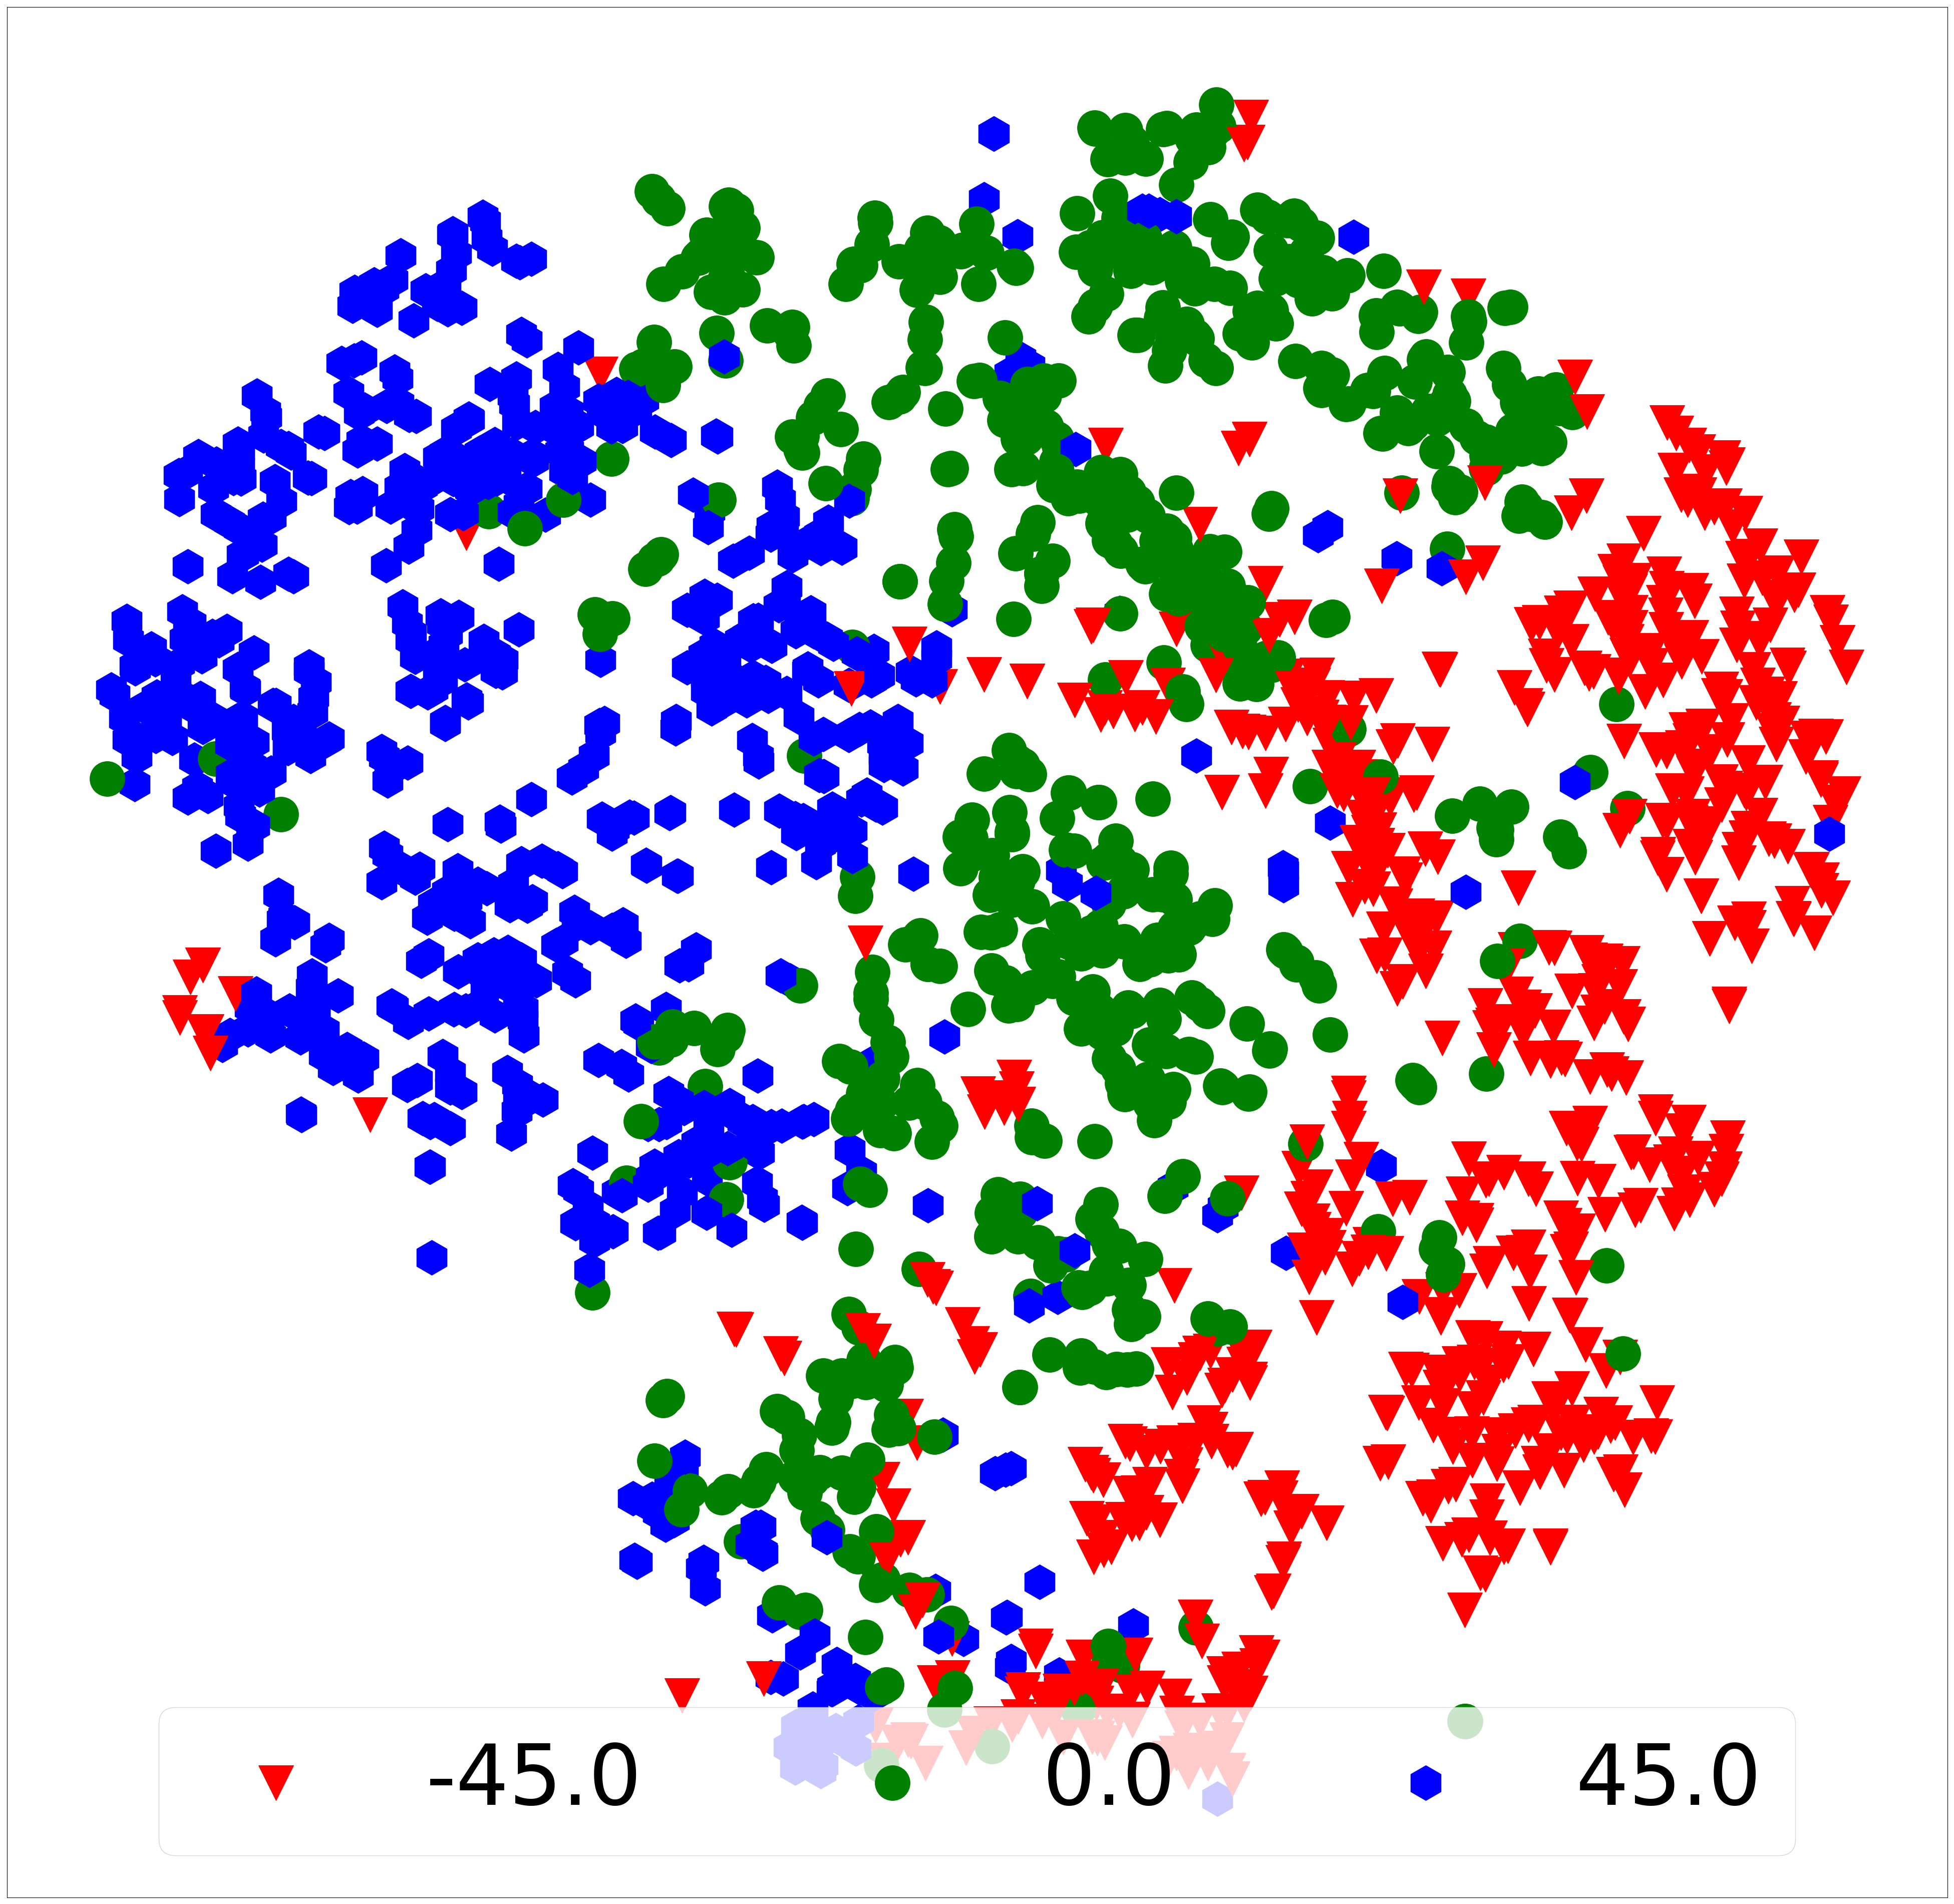
\includegraphics[width=\textwidth]{img/mnist_rot_raw_label.png}
% \caption{}
% \end{subfigure}
% \hspace{0.1\textwidth}
% \begin{subfigure}{.275\textwidth}
% \centering
% 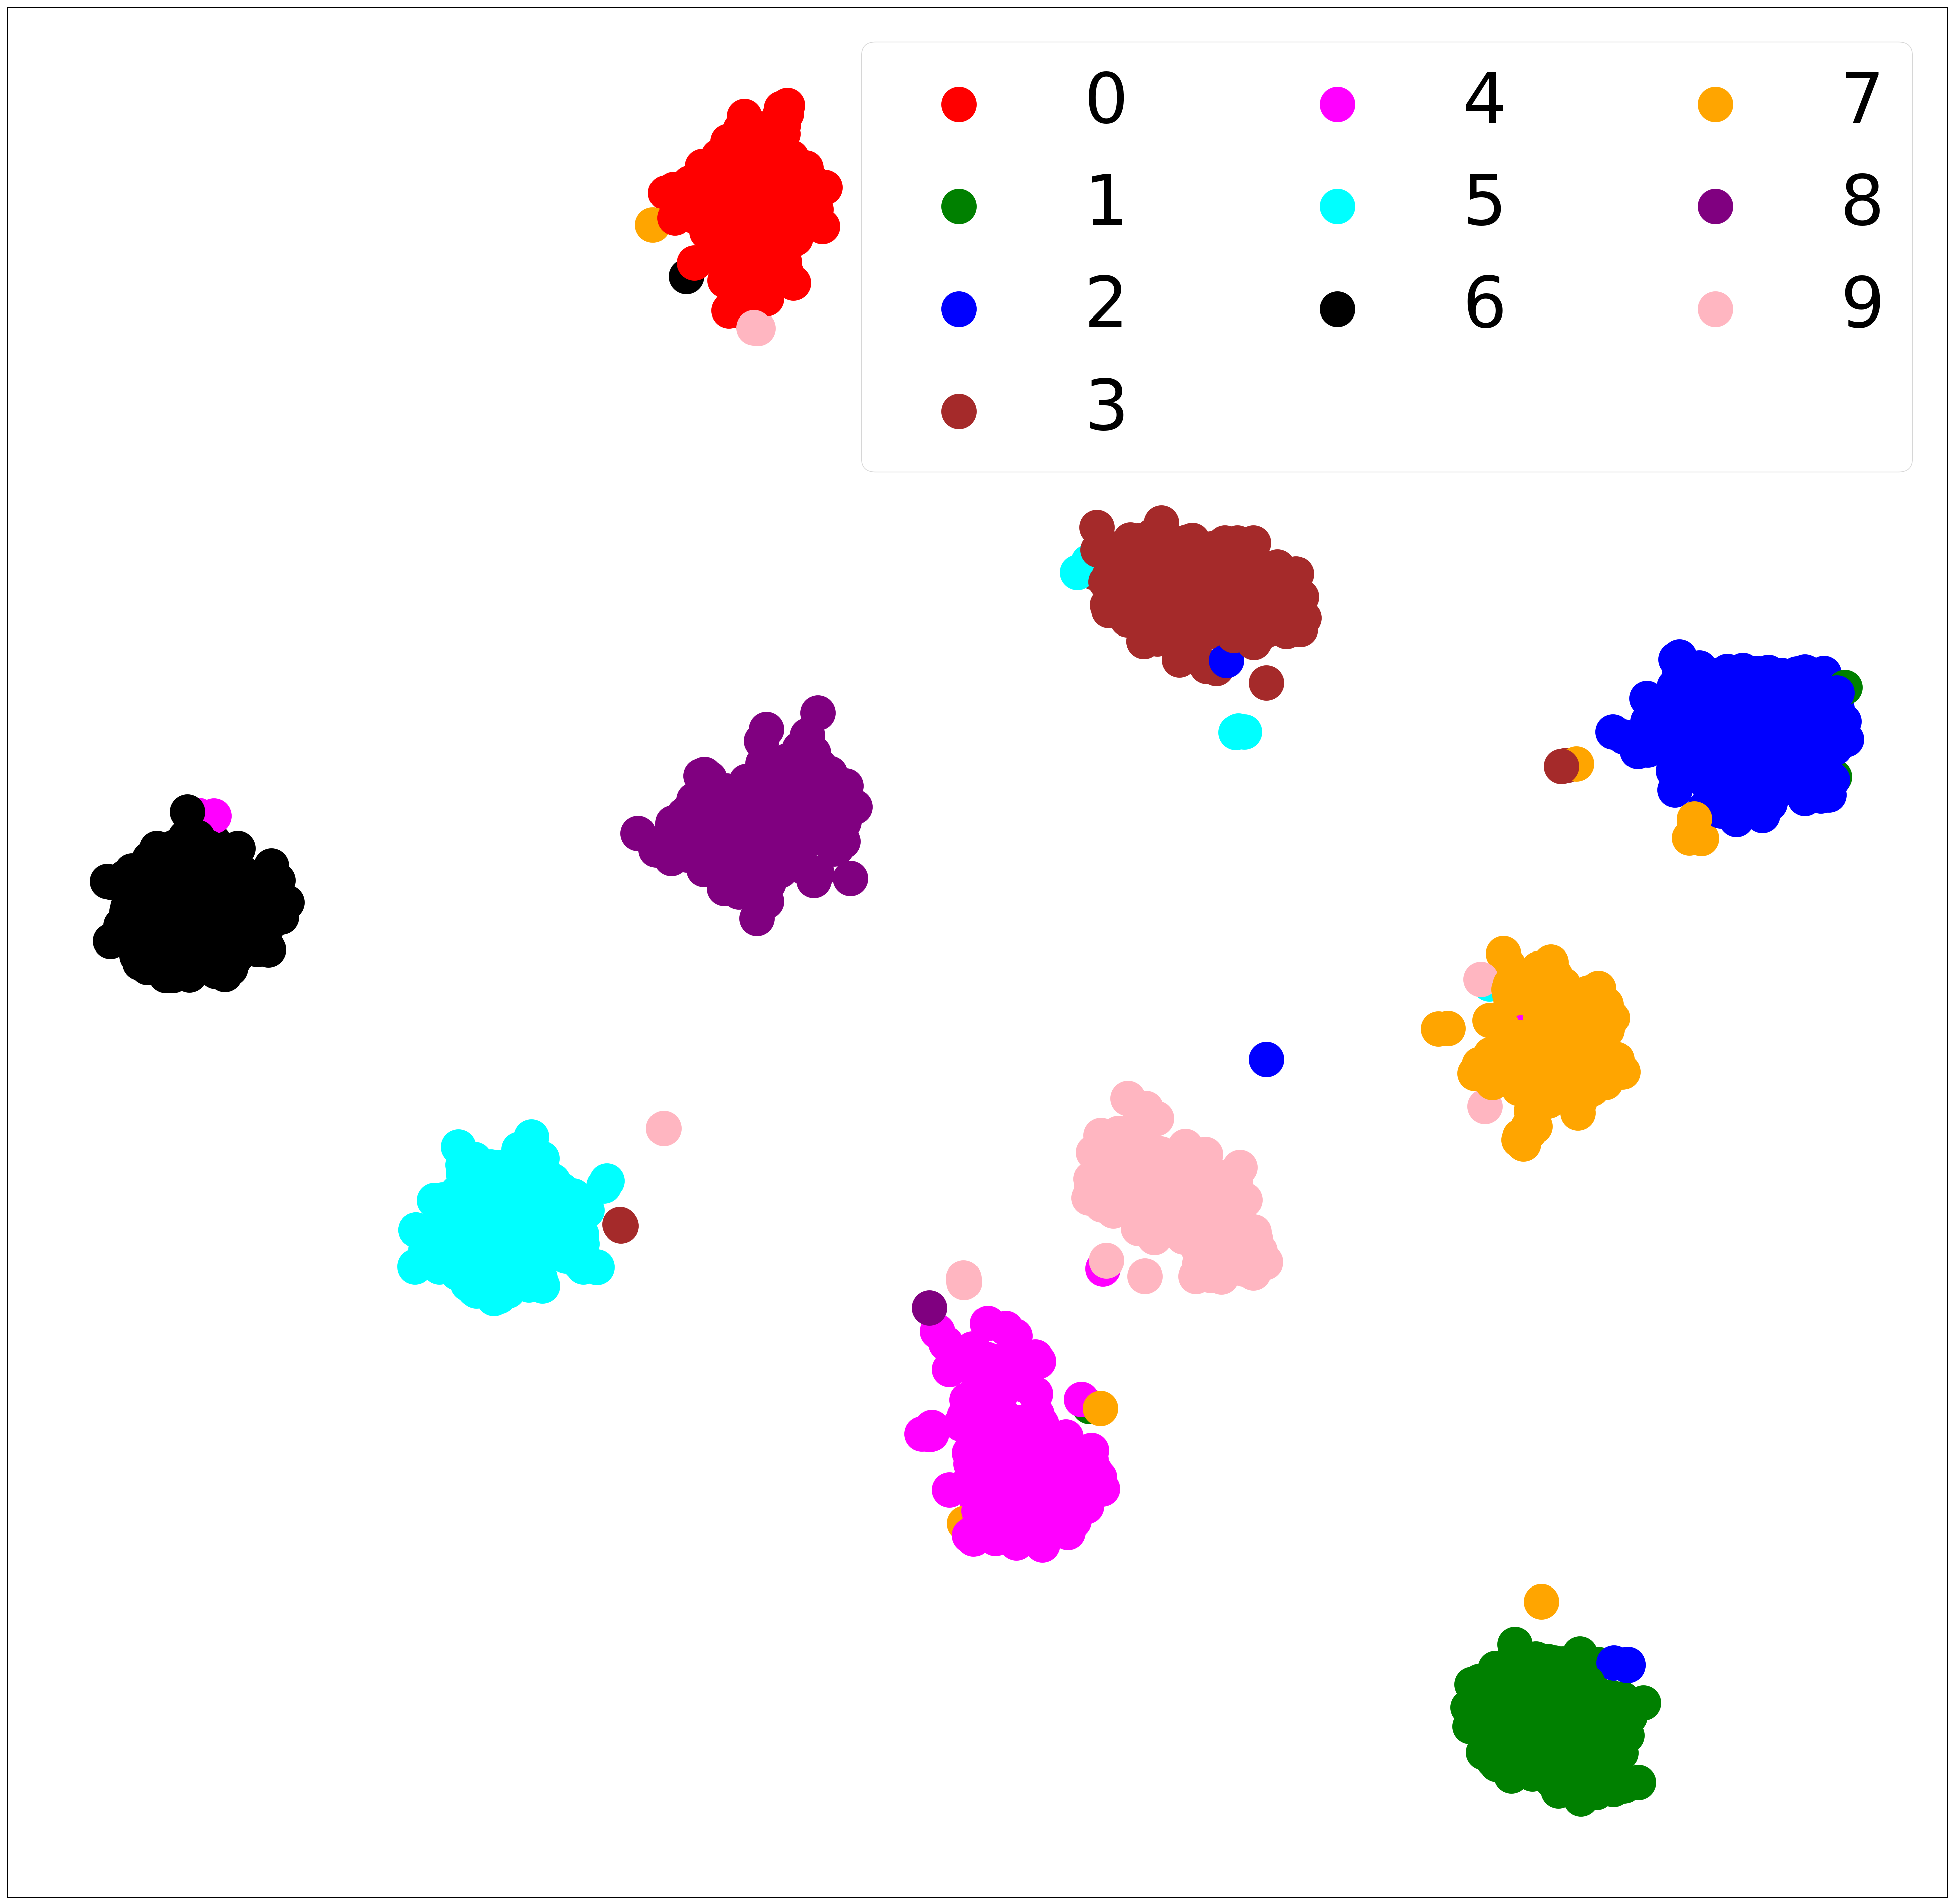
\includegraphics[width=\textwidth]{img/mnist_rot_e1_label.png}
% \caption{}
% \end{subfigure}
% \caption{MNIST-ROT -- t-SNE visualization of (a) raw data and (b) $e_1$ labeled by digit-class}
% \label{fig:tsne_mnist_rot}
% \end{figure}


\makegapedcells
\begin{table}
\centering

% \begin{minipage}[c]{0.23\textwidth}
% \centering
% \small
% \begin{tabular}{ c ?{1.5pt} c ?{1.5pt} c }
%   \hbline
%   \nocell{1} & \textbf{CAI} & \textbf{Ours} \\
%   \hbline
%   $A_y$ & 0.68 & \textbf{0.74} \\
%   $A_z$ & 0.66 & \textbf{0.0} \\
%   \hbline
% \end{tabular}
% \vspace{3pt}
% \captionof{table}{\label{tab:chairs}Results on Chairs}
% \end{minipage}
% \hspace{5pt}
\begin{minipage}[c]{0.43\textwidth}
\centering
\small
\begin{tabular}{ c ?{1.5pt} c ?{1.5pt} c ?{1.5pt} c ?{0.25pt} c ?{0.25pt} c }
  \hbline
  \textbf{Metric} & \textbf{Angle} & \textbf{CAI} & \textbf{Ours} & $\boldsymbol{B_0}$ & $\boldsymbol{B_1}$ \\
  \hbline
  &&&&& \\ [-2.5ex]
  \multirow{3}*{$A_y$}& $\Theta$ & 0.958 & \textbf{0.977} & 0.974 & 0.972 \\
  & $\pm 55^{\degree}$ & 0.826 & \textbf{0.856}  & 0.826 & 0.829 \\
  & $\pm 65^{\degree}$ & 0.662 & \textbf{0.696} & 0.674 & 0.682 \\
  \hbline
  $A_z$ & - & 0.384 & \textbf{0.338} & 0.586 & 0.409 \\
  \hbline
\end{tabular}
\vspace{3pt}
\captionof{table}{\label{tab:mnist_rot}Results on MNIST-ROT. $\Theta = \{0, \pm 22.5^{\degree}, \pm 45^{\degree}\}$ was used for training. High $A_y$ and low $A_z$ are desired.}
\end{minipage}
\hfill
\begin{minipage}[c]{0.44\textwidth}
\makegapedcells
\centering
\small
\begin{tabular}{ c ?{1.5pt} c ?{1.5pt} c ?{0.25pt} c ?{0.25pt} c }
  \hbline
  $\boldsymbol{k}$ & \textbf{CAI} & \textbf{Ours} & $\boldsymbol{B_0}$ & $\boldsymbol{B_1}$ \\
  \hbline
  -2 & 0.816 & \textbf{0.880} & 0.872 & 0.870 \\
  2 & 0.933 & \textbf{0.958} & 0.942 & 0.940 \\
  3 & 0.795 & \textbf{0.874} & 0.847 & 0.853 \\
  4 & 0.519 & \textbf{0.606} & 0.534 & 0.550 \\
  \hbline
\end{tabular}
\vspace{3pt}
\captionof{table}{\label{tab:mnist_dil}MNIST-DIL -- Accuracy of predicting $y$ ($A_y$). $k = -2$ \ represents erosion with kernel-size of $2$.}
\end{minipage}
% \hfill
% \begin{minipage}{0.28\textwidth}
% \centering

% \small
% \begin{tabular}{ c ?{1.5pt} c ?{0.25pt} c ?{0.25pt} c }
%   \hbline
%   \textbf{CAI} & \textbf{Ours} & $\boldsymbol{B_0}$ & $\boldsymbol{B_1}$ \\
%   \hbline
%   0.333 & \textbf{0.231} & 0.659 & 0.452 \\
%   \hbline
% \end{tabular}
% \vspace{5pt}
% \caption{\label{tab:mnist_rot_z}MNIST-ROT -- Accuracy of predicting $z$ from $e_1$ ($A_z$)}

% \end{minipage}

\end{table}

% \begin{figure}
% \captionsetup[subfigure]{font=scriptsize,labelfont=scriptsize,aboveskip=-1pt,belowskip=1pt}
% \centering
% \begin{subfigure}{.25\textwidth}
% \centering
% \includegraphics[trim={0 0 0 0.75cm},clip,width=0.9\textwidth]{img/mnist_recon_e1.png}
% \caption{}
% \end{subfigure}
% \begin{subfigure}{.25\textwidth}
% \centering
% \includegraphics[trim={0 0 0 0.75cm},clip,width=0.9\textwidth]{img/mnist_recon_e2.png}
% \caption{}
% \end{subfigure}
% \begin{subfigure}{.25\textwidth}
% \centering
% \includegraphics[trim={0 0 0 0.75cm},clip,width=0.9\textwidth]{img/mnist_recon_e1e2.png}
% \caption{}
% \end{subfigure}
% \caption{MNIST-ROT -- reconstruction from (a) $e_1$, (b) $e_2$ and (c) $e = [e_1 \ e_2]$. Alternate columns show real and reconstructed images.}
% \label{fig:recon_mnist_rot}
% \end{figure}

% \makegapedcells
% \begin{table}
% \centering
% \caption{MNIST-DIL -- Accuracy of predicting $y$ from $e_1$ ($A_y$). Models were trained on MNIST-ROT.}
% \label{tab:mnist_dil}
% \small
% \begin{tabular}{ c ?{1.5pt} c ?{1.5pt} c ?{0.25pt} c ?{0.25pt} c }
%   \hbline
%   \textbf{Dilation kernel-size ($\boldsymbol{k}$)} & \textbf{CAI} & \textbf{Ours} & $\boldsymbol{B_0}$ & $\boldsymbol{B_1}$ \\
%   \hbline
%   -2 (erosion with $k$ = 2) & 0.8161 & \textbf{0.8804} & 0.8717 & 0.8703 \\
%   2 & 0.9326 & \textbf{0.9581} & 0.9416 & 0.9403 \\
%   3 & 0.7953 & \textbf{0.8740} & 0.8470 & 0.8531 \\
%   4 & 0.5188 & \textbf{0.6064} & 0.5335 & 0.5500 \\
%   \hbline
% \end{tabular}
% \end{table}


% \subsubsection{MNIST-ROT}

% \vspace{10pt}
\textbf{MNIST-ROT.\quad} We create this variant of the MNIST dataset by randomly rotating each image by an angle $\theta \in \{-45^{\degree}, -22.5^{\degree}, 0^{\degree}, 22.5^{\degree}, 45^{\degree}\}$ about the Y-axis. We denote this set of angles as $\Theta$. The angle information is used as a one-hot encoding while training the CAI model. We evaluate all the models on the same metrics $A_y$ and $A_z$ we previously used. We additionally test all the models on $\theta \not \in \Theta$ to gauge the performance of these models on unseen variations of the rotation nuisance factor. Table~\ref{tab:mnist_rot} summarizes the results, showing that our unsupervised adversarial model not only performs better than the baseline ablation versions but also outperforms CAI, which uses supervised information about the rotation angle. The difference in $A_y$ is especially notable for the cases where $\theta \not \in \Theta$. Results on $A_z$ show that our model discards more information about $\theta$ than CAI even though CAI uses $\theta$ information during training. The information about $\theta$ migrates to $e_2$, indicated by the accuracy of predicting it from $e_2$ being $0.77$. Figure~\ref{fig:tsne_mnist_rot} shows t-SNE visualization of raw MNIST-ROT images and $e_1$ learned by our model. While raw data tends to cluster by the rotation angle, $e_1$ shows near-perfect grouping based on the digit-class. We further visualize the $e_1$ embedding learned by the proposed model and the baseline $B_0$, which models the classifier $x \dashedrightarrow h \dashedrightarrow y$, to investigate the effectiveness of invariance induction by exclusion versus inclusion, respectively. Both the models were trained on digits rotated by $\theta \in \Theta$ and  t-SNE visualizations were generated for $\theta \in \{\pm55\}$. Figure~\ref{fig:e1_55} shows the results. As evident, $e_1$ learned by the proposed model shows no clustering by the rotation angle, while that learned by $B_0$ does, with encodings of some digit classes forming multiple clusters corresponding to rotation angles. Figure~\ref{fig:recon_mnist_rot} shows results of reconstructing $x$ from $e_1$ and $e_2$ generated in the same way as Extended Yale-B above. The figures show that reconstructions from $e_1$ reflect the digit class but contain no information about $\theta$, while those from $e_2$ exhibit the inverse.

% \begin{minipage}{\textwidth}
% \centering
% \begin{minipage}[c]{0.58\textwidth}
\begin{figure}
% \vspace{-15pt}
\centering
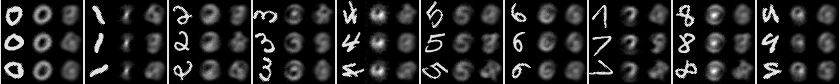
\includegraphics[width=\textwidth]{img/mnist_recon.png}
\caption{MNIST-ROT -- reconstruction from $e_1$ and $e_2$, (c) $e$.  Columns in each block reflect (left to right): real, reconstruction from $e_1$ and that from $e_2$.}
\label{fig:recon_mnist_rot}
\end{figure}
% \end{minipage}
% \hfill
% \begin{minipage}[c]{0.40\textwidth}
% \makegapedcells
% \centering
% \small
% \begin{tabular}{ c ?{1.5pt} c ?{1.5pt} c ?{0.25pt} c ?{0.25pt} c }
%   \hbline
%   $\boldsymbol{k}$ & \textbf{CAI} & \textbf{Ours} & $\boldsymbol{B_0}$ & $\boldsymbol{B_1}$ \\
%   \hbline
%   -2 & 0.816 & \textbf{0.880} & 0.872 & 0.870 \\
%   2 & 0.933 & \textbf{0.958} & 0.942 & 0.940 \\
%   3 & 0.795 & \textbf{0.874} & 0.847 & 0.853 \\
%   4 & 0.519 & \textbf{0.606} & 0.534 & 0.550 \\
%   \hbline
% \end{tabular}
% \vspace{5pt}
% \captionof{table}{MNIST-DIL -- Accuracy of predicting $y$ from $e_1$ ($A_y$). Models were trained on MNIST-ROT. $k = -2$ represents erosion.}
% \label{tab:mnist_dil}
% \end{minipage}
% \end{minipage}

% \subsubsection{MNIST-DIL}

% \vspace{10pt}
\textbf{MNIST-DIL.\quad} We create this variant of MNIST by eroding or dilating MNIST digits using various kernel-sizes ($k$). We use models trained on MNIST-ROT to report evaluation results on this dataset, to show the advantage of unsupervised invariance induction in cases where certain $z$ are not annotated in the training data. Thus, information about these $z$ cannot be used to train supervised invariance induction models. We also provide ablation results on this dataset using the same baselines $B_0$ and $B_1$. Table~\ref{tab:mnist_dil} summarizes the results of this experiment. The results show significantly better performance of our model compared to CAI and the baselines. More notably, CAI performs \emph{significantly} worse than our baseline models, indicating that the supervised approach of invariance induction can worsen performance with respect to nuisance factors not accounted for during training.


\subsection{Domain Adaptation}

Domain adaptation has been treated as an invariance induction task in recent literature~\cite{bib:dann,bib:vfae} where the goal is to make the prediction task invariant to the ``domain'' information. We evaluate the performance of our model at domain adaptation on the Amazon Reviews dataset~\cite{bib:amzrev} using the same preprocessing as~\cite{bib:vfae}. The dataset contains text reviews on products in four domains -- ``books'', ``dvd'', ``electronics'', and ``kitchen''. Each review is represented as a feature vector of unigram and bigram counts. The target $y$ is the sentiment of the review -- either positive or negative. We use the same experimental setup as~\cite{bib:dann,bib:vfae} where the model is trained on one domain and tested on another, thus creating $12$ source-target combinations. We design the architectures of the encoder and the decoder in our model to be similar to those of VFAE, as presented in~\cite{bib:vfae}. Table~\ref{tab:amzrev} shows the results of the proposed unsupervised adversarial model and supervised state-of-the-art methods VFAE and Domain Adversarial Neural Network (DANN)~\cite{bib:dann}. The results of the prior works are quoted directly from~\cite{bib:vfae}. The results show that our model outperforms both VFAE and DANN at nine out of the twelve tasks. Thus, our model can also be used effectively for domain adaptation.

\makegapedcells
\begin{table}
\centering
\small
\begin{tabular}{ c ?{1.5pt} c ?{0.75pt} c ?{0.75pt} c } % ?{1.5pt} c ?{0.75pt} c }
  \hbline
  % \textbf{Source - Target} & \multicolumn{3}{c ?{1.5pt}}{$\boldsymbol{A_y}$} & \multicolumn{2}{c}{$\boldsymbol{A_z}$} \\
  % \Cline{2.5\arrayrulewidth}{2-6}
  \textbf{Source - Target} & \textbf{DANN~\cite{bib:dann}} & \textbf{VFAE~\cite{bib:vfae}} & \textbf{Ours} \\ % & \textbf{VFAE~\cite{bib:vfae}} & \textbf{Ours} \\
  \hbline
  books - dvd & 0.784 & 0.799 & \textbf{0.820} \\ % & 0.535 & 0.591 \\
  books - electronics & 0.733 & \textbf{0.792} & 0.764 \\ % & 0.541 & 0.636 \\
  books - kitchen & 0.779 & \textbf{0.816} & 0.791 \\ % & 0.537 & 0.629 \\
  \hline
  dvd - books & 0.723 & 0.755 & \textbf{0.798} \\ % & 0.537 & 0.591 \\
  dvd - electronics & 0.754 & 0.786 & \textbf{0.790} \\ % & 0.538 & 0.644 \\
  dvd - kitchen & 0.783 & 0.822 & \textbf{0.826} \\ % & 0.543 & 0.667 \\
  \hline
  electronics - books & 0.713 & 0.727 & \textbf{0.734} \\ % & 0.562 & 0.640 \\
  electronics - dvd & 0.738 & \textbf{0.765} & 0.740 \\ % & 0.556 & 0.670 \\
  electronics - kitchen & 0.854 & 0.850 & \textbf{0.890} \\ % & 0.536 & 0.564 \\
  \hline
  kitchen - books & 0.709 & 0.720 & \textbf{0.724} \\ % & 0.560 & 0.634 \\
  kitchen - dvd & 0.740 & 0.733 & \textbf{0.745} \\ % & 0.561 & 0.664 \\
  kitchen - electronics & 0.843 & 0.838 & \textbf{0.859} \\ % & 0.533 & 0.567 \\
  \hbline
\end{tabular}
\vspace{3pt}
\caption{\label{tab:amzrev}Results on Amazon Reviews dataset -- Accuracy of predicting $y$ from $e_1$ ($A_y$)}
\vspace{-20pt}
\end{table}